\author{João Gonçalves}
\newcommand{\authorr}{Teresa Nogueira}
\newcommand{\studentID}{99995}
\newcommand{\studentIDD}{100029}
%\newcommand{\supervisorone}{Prof\textsuperscript{\underline{a}}. XXXXXX}
\newcommand{\supervisorone}{}
\newcommand{\supervisortwo}{}
\newcommand{\department}{Engenharia Eletrotécnica e de Computadores}
\newcommand{\exam}{Modelação e Simulação}

\title{%
Apontamentos de MSim \\
\large (Alguns tópicos \href{https://github.com/Kons-5}{\raisebox{0 em}{\large \faGithub}})}
\date{Janeiro 2023}

\documentclass[a4paper,12pt]{article}
\usepackage[left=28mm,top=25mm,right=28mm,bottom=24mm]{geometry}
\usepackage[flushmargin,hang,bottom,multiple]{footmisc}
\usepackage{etoolbox}
\usepackage{fontawesome5}
\usepackage{pgfplots}
\usepackage{circuitikz}
\usepackage{booktabs}
\usepackage[usestackEOL]{stackengine}
\usepackage[T1]{fontenc}
\usepackage[utf8]{inputenc}
\usepackage{bm}
\usepackage[export]{adjustbox}
\usepackage{graphicx}
\usepackage[font=footnotesize]{caption}
\usepackage[justification=centering]{subcaption}
\usepackage{amsmath}
\usepackage{amsfonts}
\usepackage{mathtools}
\usepackage{float}
\usepackage[linktoc=all]{hyperref}
\usepackage[capitalise]{cleveref}
\usepackage{enumitem,kantlipsum}
\usepackage[square,numbers,sort]{natbib}
\usepackage[ruled,vlined]{algorithm2e}
\usepackage{listings}
\usepackage[numbered,framed]{matlab-prettifier}
\usepackage{minted}
\usepackage{amssymb}
\usepackage{babel}
\usepackage[nottoc,numbib]{tocbibind}
\usepackage{tcolorbox}
\usepackage{xcolor}
\usepackage{graphicx,array}
\usepackage{animate}
\usepackage{breakurl}
\usepackage{placeins}
\usepackage{colortbl}
\usepackage{attrib}
\usepackage{wrapfig}
\usepackage{mathabx}
\usepackage{fancyhdr}
\usepackage{amsmath}
\usepackage{lipsum}
\usepackage{textcomp}
\usepackage{physics}
\usepackage[framemethod=TikZ]{mdframed}
%\tcbuselibrary{skins,breakable}
%\usetikzlibrary{shadings,shadows}
\usemintedstyle{emacs}
\linespread{1}
%\setlength{\parindent}{0pt}

\usepackage{multimedia}

\newenvironment{block}[1]{%
    \tcolorbox[beamer,%
    noparskip,breakable,
    colback=LightBlue,colframe=DarkBlue,%
    colbacklower=DarkBlue!75!LightBlue,%
    title=#1]}%
    {\endtcolorbox}

\hypersetup{
    colorlinks,
    linkcolor={black},
    citecolor={blue!50!black},
    urlcolor={blue!50!black}
}

\lstset{
  style              = Matlab-editor,
  basicstyle         = \scriptsize\mlttfamily,
  escapechar         = ",
  mlshowsectionrules = true,
  extendedchars=true,
  literate= {á}{{\'a}}1 {é}{{\'e}}1 {í}{{\'i}}1 {ó}{{\'o}}1 {ú}{{\'u}}1 {ç}{{\c c}}1 {ã}{{\~a}}1 {õ}{{\~o}}1
  {Á}{{\'A}}1 {É}{{\'E}}1 {Í}{{\'I}}1 {Ó}{{\'O}}1 {Ú}{{\'U}}1 {Ã}{{\~A}}1,
}

%//==============================--@--==============================//%
%                         -> error messages <-                        %
\usepackage{pifont,mdframed}

\newenvironment{warning}
  {\par\begin{mdframed}[linewidth=1.5pt,linecolor=red]%
    \begin{list}{}{\leftmargin=0.9cm
                   \labelwidth=\leftmargin}\item[\raisebox{-0.4 em}{\Large\ding{43}}]}
  {\end{list}\end{mdframed}\par}

%//==============================--@--==============================//%
%                   -> reduzir espaço entre itens <-                  %
\usepackage{enumitem}
%\setlist[itemize]{nosep}
%\setlist[enumerate]{nosep}
\setlist[itemize]{itemsep=0.0125em}
\setlist[enumerate]{itemsep=0.0125em}
%//==============================METH-==============================//%
\newcounter{theo}[section]\setcounter{theo}{0}
\renewcommand{\thetheo}{\arabic{theo}}

%\definecolor{tempcolor}{RGB}{113, 110, 97}
\definecolor{tempcolor}{RGB}{0, 0, 0}
\newenvironment{theo}[2][]{%
    \refstepcounter{theo}
    \ifstrempty{#1}%
    % if condition (without title)
    {\mdfsetup{%
        frametitle={%
            \tikz[baseline=(current bounding box.east),outer sep=0pt]
            \node[anchor=east,rectangle,fill=blue!20]
            {\strut Teorema~\thetheo};}
        }%
    % else condition (with title)
    }{\mdfsetup{%
        frametitle={%
            \tikz[baseline=(current bounding box.east),outer sep=0pt]
            \node[anchor=east,rectangle,fill=white]
            {\strut #1};}%
        }%
    }%
    % Both conditions
    \mdfsetup{%
        innertopmargin=0pt,linecolor=tempcolor,%
        linewidth=2pt,topline=true,%
        frametitleaboveskip=1.25\dimexpr-\ht\strutbox\relax%
    }
 
\begin{mdframed}[]\relax\vspace{-0.5em}}{%
\end{mdframed}}

\def\delequal{\mathrel{\ensurestackMath{\stackon[1pt]{=}{\scriptstyle\Delta}}}}
%------------------------------------ MAGIC--------------------------------------
\def\UrlBreaks{\do\/\do-}
\expandafter\def\expandafter\UrlBreaks\expandafter{\UrlBreaks\do\a%
\do\b\do\c\do\d\do\e\do\f\do\g\do\h\do\i\do\j\do\k\do\l\do\m\do\n%
\do\o\do\p\do\q\do\r\do\s\do\t\do\u\do\v\do\w\do\x\do\y\do\z\do\&}

\newcolumntype{C}[1]{>{\centering\let\newline\\\arraybackslash\hspace{0pt}}m{#1}}
\newcolumntype{L}[1]{>{\raggedright\let\newline\\\arraybackslash\hspace{0pt}}m{#1}}
%----------------------------------TITLE PAGE -----------------------------------
\makeatletter
\def\maketitle{
  \begin{center}\leavevmode
        \normalfont
        
\includegraphics[width=0.5\columnwidth]{img/title-page/IST.pdf}
        \vskip 0.05cm   
        \textsc{\large \department}\\
        \vskip 0.5cm
        \rule{0.95\linewidth}{0.2 mm} %\\
        {\large \exam}\\[0.5 cm]
        {\huge \bfseries \@title \par} 
        \vspace{1em}
        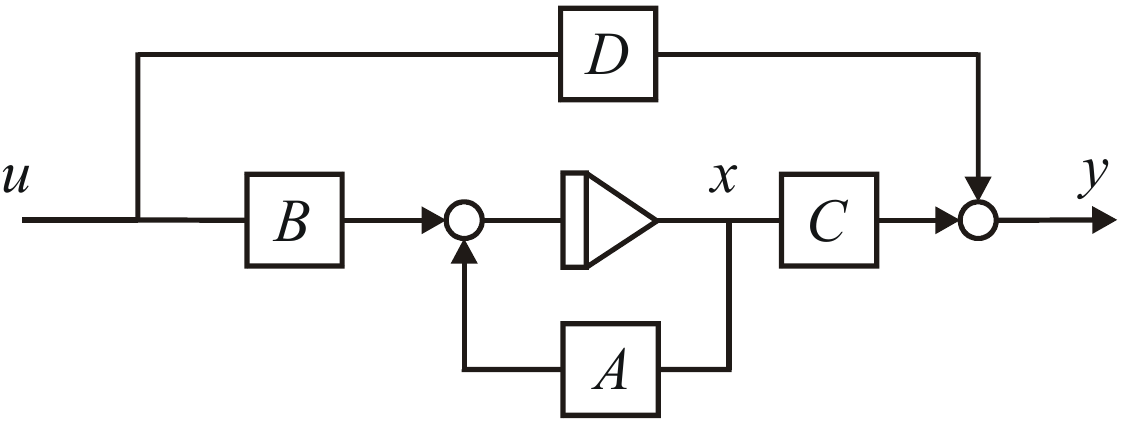
\includegraphics[scale=1]{img/title-page/000.png}
        \vspace{-0.5em}
        \captionof*{figure}{\color{gray} Imagem: \textit{Linear time-invariant state space model} (Egeland \& Gravdahl 2002)}
        %\vspace{0.5cm}
        \rule{0.95\linewidth}{0.2 mm} \\[0.75 cm]
        %\fontsize{9pt}{11pt}\selectfont
        \begin{minipage}[t]{1\textwidth}
	   \begin{flushleft} \large
                \emph{Autores:}\\
			\normalsize \textbf{\@author} : \studentID\\
                \fontsize{9pt}{11pt}\selectfont $\hookrightarrow$ jrazevedogoncalves@tecnico.ulisboa.pt \\
                \normalsize \textbf{\authorr} : \studentIDD\\
                \scriptsize $\hookrightarrow$ maria.teresa.ramos.nogueira@tecnico.ulisboa.pt
		\end{flushleft}
	\end{minipage}
	\vfill
	{\Large \@date\par}
   \end{center}
   %\vfill
   %\null
   \cleardoublepage
  }
\makeatother
%-------------------------------- ENDTITLE PAGE ----------------------------------
%---> Header <---
%\fancyhf{}
\renewcommand{\headrulewidth}{1pt}% Header rule width
\renewcommand{\footrulewidth}{0pt}% No footer rule
\setlength\headheight{26pt} 
\fancyhead[L]{\raisebox{0.1\height}[0pt][0pt]{\textit{Modelação e Simulação}}}
\fancyhead[R]{\raisebox{0.1\height}[0pt][0pt]{2022/2023}}

\pgfplotsset{compat=1.18}
\setcounter{tocdepth}{4}
%\setcounter{secnumdepth}{4}
\setcounter{secnumdepth}{-2}

\renewcommand{\figurename}{Fig.}
\renewcommand{\tablename}{Tab.}
\renewcommand{\contentsname}{Índice}
\settocbibname{\raisebox{0em}{Referências}}
\setlength{\bibsep}{0.1em}%reduzir espaço entre refs.

%\renewcommand{\bibpreamble}{\vspace{-8em}}
\usepackage[titles]{tocloft}

\setlength{\cftbeforesecskip}{0.25em}

\usepackage{pdfpages}
\begin{document}
    \sloppy
    %% title page
    \pagenumbering{gobble}
    \maketitle
    %% toc
    \tableofcontents
    %% body
    \newpage
    \pagestyle{fancy}
    \pagenumbering{arabic}
    % %\phantomsection\addcontentsline{toc}{section}{}\vskip -0em%
    %     \input{src/Intro}

    \clearpage
    \section{1. Modelos de Espaço de Estados e Análise do Modelo}
        %//==============================--@--==============================//%
\subsection[1.1 Modelos de espaço de estados]{$\rightarrow$ Modelos de espaço de estados\cite{Lemos2019}}
\label{subsec:state-space-model}

%Cutie, à escuta? adoro-te :3 %amo-te muito, descansa

\noindent No caso geral, para \underline{Sistemas Lineares Contínuos} temos:
\begin{align*}
    \dot{\pmb{x}}(t) &= \pmb{A}\, \pmb{x}(t) + \pmb{B}\, \pmb{u}(t)\qquad \pmb{x}(t_0) = \pmb{x}_0 \\
    \pmb{y}(t) &= \pmb{C}\, \pmb{x}(t) + \pmb{D}\, \pmb{u}(t)
\end{align*}

\noindent Em que as matrizes são:
\begin{enumerate}\footnotesize
    \item[$\blacktriangle$] $\pmb{A}$ - Matriz da Dinâmica (\underline{quadrada}) - Define o comportamento dinâmico do Sistema, i.e. se é instável ou estável, e se é rápido ou lento. Essas características dependem dos \underline{valores próprios}.
    \item[$\blacktriangle$] $\pmb{B}$ - Matriz da Entrada (normalmente \underline{matriz coluna}) - Define o modo como a entrada (actuação) afeta o estado.
    \item[$\blacktriangle$] $\pmb{C}$ - Matriz de Saída (normalmente \underline{matriz linha}) - É a relação entre o estado do sistema e a saída que se deseja escolher.
    \item[$\blacktriangle$] $\pmb{D}$ - Matriz de Saída direta (normalmente \underline{nula}) - Define o modo como a entrada (actuação) afeta diretamente a saída; \underline{para sistemas causais é nula}.
\end{enumerate}

\noindent E os domínios são:
\begin{enumerate}\footnotesize
    \item[$\blacktriangle$] Estados: $\pmb{x}(t)\in \mathbb{R}^n$ em que $n =$ \#estados (também chamada \underline{ordem do sistema}) %adoro-te; muitos miminhos armazenados <3 ahhhh, adorava estar aí
    \item[$\blacktriangle$] Entradas: $\pmb{u}(t)\in \mathbb{R}^m$ em que $m =$ \#entradas (\underline{normalmente 1})
    \item[$\blacktriangle$] Saídas: $\pmb{y}(t)\in \mathbb{R}^p$ em que $p =$ \#saídas (\underline{normalmente 1})
\end{enumerate}

\noindent Como tal, as matrizes têm as seguintes dimensões:
$$
    \pmb{A}\, [n\times n]\quad \pmb{B}\, [n\times m]\quad \pmb{C}\, [p\times n]\quad \pmb{D}\, [p\times m]\qquad\left[ \begin{array}{c|c} \pmb{A} & \pmb{B} \\ \midrule \pmb{C} & \pmb{D} \\ \end{array}\right]
$$

\noindent Desta forma, o Modelo em Espaço de Estados toma a seguinte representação:
\begin{figure}[H]
    \centering
    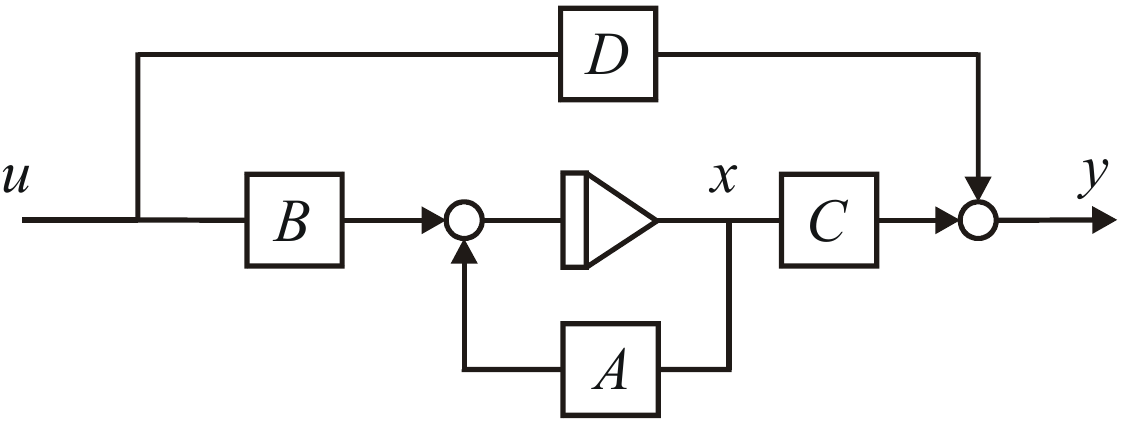
\includegraphics[width = 0.85\linewidth]{img/state-space-models/LTI-state-space-model.png}
    \caption{Representação em Diagrama de Blocos do Modelo em Espaço de Estados (LIT).}
    \label{fig:LTI-state-space-model}
\end{figure}

%//==============================--A--==============================//%
\newpage
\subsubsection[1.1.1 Conversão entre Modelo de Estado e Função de Transferência]{$\pmb{\rightarrow}$ Conversão entre Modelo de Estado e Função de Transferência}
\label{subsec:convertion-to-transfer}

\noindent Partindo do Modelo em Espaço de Estados da \hyperref[subsec:state-space-model]{secção anterior}\footnotemark[1]:
\begin{align*}
    \dot{\pmb{x}}(t) &= \pmb{A}\, \pmb{x}(t) + \pmb{B}\, u(t)\qquad \pmb{x}(t_0) = \pmb{x}_0 \\
    y(t) &= \pmb{C}\, \pmb{x}(t)
\end{align*}

\noindent E aplicando a Transformada de Laplace ($\mathcal{L}\{\cdot\}$) com \underline{condições iniciais nulas}, obtém-se:
$$
    \begin{cases}
        s\pmb{X}(s) = \pmb{A}\,\pmb{X}(s) + \pmb{B}\,U(s) \\
        Y(s) = \pmb{C}\, \pmb{X}(s)
    \end{cases}
$$
$$
    \therefore Y(s) = \pmb{C}\left( s\pmb{I}-\pmb{A} \right)^{-1}\pmb{B}\,U(s)
$$

\noindent E, como tal, é possível converter novamente para tempo continuo usando a Transformada de Laplace Inversa ($\mathcal{L}^{-1}\{\cdot\}$), i.e.:
$$
    y(t) = \mathcal{L}^{-1}\{\pmb{C}\left( s\pmb{I}-\pmb{A} \right)^{-1}\pmb{B}\,U(s)\}
$$

\vspace{-0.5em}
{
\mdfsetup{linewidth=2pt}

\begin{mdframed}
    \noindent Esta análise também permite definir a \underline{Função de Transferência} (relação da entrada com a saída):
    
    \vspace{-0.5em}
    $$
        G(s) \delequal \frac{Y(s)}{U(s)} = \pmb{C}\left( s\pmb{I}-\pmb{A} \right)^{-1}\pmb{B},
    $$
\end{mdframed}
}

\noindent em que
$$
    \left( s\pmb{I}-\pmb{A} \right)^{-1} = \frac{\text{adj}\left[(s\pmb{I}-\pmb{A}) \right]}{\det\left[( s\pmb{I}-\pmb{A}) \right]}
$$

{
\mdfsetup{linewidth=2pt}

\begin{mdframed}
    \noindent $\pmb{\rightarrow}$ \textbf{\textit{Nota}:} As soluções obtidas resultam do facto da \underline{condição inicial ser nula}. Caso não se verificasse, não seria possível deduzir uma Função de Transferência, e ter-se-ia ainda:
    \vspace{-0.5em}
    $$
        y(t) = \mathcal{L}^{-1}\{\pmb{C}\left( s\pmb{I}-\pmb{A} \right)^{-1}\cdot(\pmb{x}_0+\pmb{B}\,U(s))\}
    $$
    \vskip -0.5em
    \hfill\ensuremath{\Box}
\end{mdframed}
}

\footnotetext[1]{Daqui em diante, assume-se $\pmb{D} \equiv \pmb{0}$.}
%//==============================--B--==============================//%
\vspace{-1em}
\subsubsection[1.1.2 Pólos e Zeros]{$\pmb{\rightarrow}$ Pólos e Zeros}
\label{subsec:poles-and-zeroes}

\noindent Ao analisar a Função de Transferência, é possível observar os pólos e os zeros.
\begin{enumerate}
    \item[$\blacktriangle$] Os pólos são, por definição, as raízes do \underline{denominador de $G(s)$}, o chamado polinómio característico:
\end{enumerate}
\vspace{-0.5em}
$$
    \det\left[( s\pmb{I}-\pmb{A}) \right] = 0
$$

\noindent Os pólos, neste caso, \underline{apenas} dependem da Matriz da Dinâmica. 

\begin{enumerate}
    \item[$\blacktriangle$] Os zeros são, por definição, as raízes do \underline{numerador de $G(s)$}:
\end{enumerate}
\vspace{-0.5em}
$$
    \pmb{C}\,\text{adj}\left[(s\pmb{I}-\pmb{A}) \right]\pmb{B} = 0
$$

\noindent Note-se que os zeros dependem não só da Matriz da Dinâmica mas também das Matrizes de Entrada e de Saída.
%//==============================--C--==============================//%
\newpage
\subsubsection[1.1.3 Obtenção do Modelo de Estado através da Função de Transferência]{$\pmb{\rightarrow}$ Obtenção do Modelo de Estado através da Função de Transferência}
\label{subsec:transfer-to-model}

\noindent Tendo a Função de Transferência é possível obter o Modelo de Estado. Este modelo não é único, existem infinitas realizações de modelos, que podem ser obtidas umas das outras através de transformações.

%%%%%
\paragraph[1.1.3 a) Sistema sem Zeros]{$\pmb{\star}$ Sistema sem Zeros:}\mbox{}\\
\noindent Neste caso a Função de Transferência é do tipo:
$$
    G(s) = \frac{b_0}{s^n + a_1 s^{n-1} + \dots + a_{n-1} s + a_n}
$$

\noindent Uma realização possível é utilizar as variáveis de fase, i.e., começar por definir os estados (fases) como sendo:
\vspace{-0.5em}
\begin{align*}
    x_1(t) &= y(t) \\
    x_2(t) &= \dot{x}_1(t) = \dot{y}(t) \\
           &\mkern9mu\vdots \\
    x_n(t) &= \dot{x}_{n-1}(t) = y^{(n-1)}(t)
\end{align*}

\noindent E como tal, a derivada a última variável de fase é dada por:
$$
    \dot{x}_n(t) = y^{(n)}(t) = -a_1 x_n(t) - a_2 x_{n-1}(t) \hdots - a_{n-1} x_1(t) + b_0 u(t)
$$

\noindent Ou seja, temos a Matriz da Dinâmica na \underline{forma companheira} e podemos definir um Modelo de Estados da seguinte forma:
$$
    \dot{\pmb{x}}(t) = 
    \begin{bmatrix} 
        0 & 1 & \dots & 0 & 0\\
        0 & 0 & 1 & \dots & 0\\
        \vdots &  &  & \ddots & \vdots\\
        0 & 0 & \dots & 0 & 1\\
        -a_n & -a_n & \dots & -a_2 & -a_1 
    \end{bmatrix} \pmb{x}(t) 
    + 
    \begin{bmatrix} 
        0\\
        0\\
        \vdots\\
        0\\
        b_0
    \end{bmatrix}
    u(t)
$$

\noindent E a Equação de Saída como:
$$
    y(t) = 
    \begin{bmatrix}
        1 & 0 & \dots & 0    
    \end{bmatrix}
    \pmb{x}(t)
$$

%%%%%
\paragraph[1.1.3 b) Sistema com Zeros]{$\pmb{\star}$ Sistema com Zeros:}\mbox{}\\
Neste caso a Função de Transferência é do tipo:
$$
    G(s) = \frac{b_1 s^{n-1} + b_2 s^{n-2} + \dots + b_n}{s^n + a_1 s^{n-1} + \dots + a_{n-1} s + a_n}
$$

\noindent (a equação anterior é assim definida para sistemas causais.)

É possível definir o sistema como uma parte sem zeros e outra com zeros:
\begin{enumerate}
    \item[$\blacktriangle$] Parte sem zeros: $X_1(s) = \dfrac{1}{s^n + a_1 s^{n-1} + \dots + a_{n-1} s + a_n}\cdot U(s)$
    \item[$\blacktriangle$] Parte com zeros: $Y(s) = X_1(s) \cdot (b_1 s^{n-1} + b_2 s^{n-2} + \dots + b_n)$
\end{enumerate}

\begin{figure}[H]
    \centering
    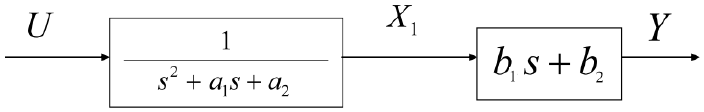
\includegraphics[width = 0.85\linewidth]{img/state-space-models/transfer-decomposition.png}
    \caption{Decomposição do sistema (LIT) numa parte com e noutra sem zeros.}
    \label{fig:transfer-decomposition}
\end{figure}

\noindent A parte \underline{sem zeros} resulta em:
$$
    \dot{\pmb{x}}(t) = 
    \begin{bmatrix} 
        0 & 1 & \dots & 0 & 0\\
        0 & 0 & 1 & \dots & 0\\
        \vdots &  &  & \ddots & \vdots\\
        0 & 0 & \dots & 0 & 1\\
        -a_n & -a_n & \dots & -a_2 & -a_1 
    \end{bmatrix} \pmb{x}(t) 
    + 
    \begin{bmatrix} 
        0\\
        0\\
        \vdots\\
        0\\
        1
    \end{bmatrix}
    u(t)
$$

\noindent E, finalmente, a parte \underline{com zeros} leva a que:
$$
    y(t) = 
    \begin{bmatrix}
        b_n & b_{n-1} & \dots & b_2 & b_1    
    \end{bmatrix}
    \pmb{x}(t)
$$

{
\mdfsetup{linewidth=2pt}

\begin{mdframed}
    \noindent $\pmb{\rightarrow}$ \textbf{\textit{Nota}:} No sistema com zeros a Matriz da Dinâmica manteve-se constante!
\end{mdframed}
}

%//==============================--D--==============================//%
\subsubsection[1.1.4 A equação homogénea e Notas sobre Álgebra Linear]{$\pmb{\rightarrow}$ A equação homogénea}
\label{subsec:homogeneous-equation}

Relaxando o Modelo do sistema para que contenha apenas a Matriz da Dinâmica, obtém-se um Sistema mais simples. A solução desta equação desempenha um papel fundamental na solução da equação de estado (de \hyperref[subsec:non-homogeneous-equation]{sistemas lineares com entrada}) e na compreensão da
dinâmica local de muitos sistemas não lineares. 

A estrutura da solução depende dos \underline{valores próprios} e dos \underline{vetores próprios} de $\pmb{A}$. Assim:
\vspace{0em}
$$
    \dot{\pmb{x}}(t) = \pmb{A}\, \pmb{x}(t)\qquad \pmb{x}(t_0) = \pmb{x}_0 \\
$$

{
\mdfsetup{linewidth=2pt}

\begin{mdframed}
    \noindent $\pmb{\rightarrow}$ \textbf{\textit{Notas sobre Álgebra Linear}:}
    
    \noindent Sendo $\pmb{A}$ quadrada $[n \times n]$, é possível chegar à seguinte igualdade:
    
    \vspace{0em}
    $$
        \pmb{A}\, \pmb{v}_i = \lambda_i\, \pmb{v}_i
    $$

    \begin{enumerate}
        \item[$\blacktriangle$] \textbf{Valores próprios:} $\lambda_i$ são as soluções de $\det[(\lambda\pmb{I}-\pmb{A})] = 0$.

        \item[$\blacktriangle$] \textbf{Vetores próprios:} $\pmb{v}_i$ são as soluções de $(\lambda_i\pmb{I}-\pmb{A})\pmb{v}_i = 0$ (são definidos a menos de uma razão de normalização).
    \end{enumerate}

    \noindent Em que $\pmb{v}_i$ também se pode denominar por \underline{vetor de modo}. Geralmente existem (podem não existir) $n$ vetores próprios linearmente independentes. Caso existam podemos utilizar a \underline{diagonalização de matrizes} para resolver a equação homogénea (veremos em seguida).
\end{mdframed}
}

\newpage

{
\mdfsetup{linewidth=2pt}

\begin{mdframed}
    \noindent $\pmb{\rightarrow}$ \textbf{\textit{Diagonalização de matrizes}:}

    \noindent Tendo $n$ vetores próprios linearmente independentes então é possível definir a Matriz Modal $[n \times n]$, não singular (admite inversa):
    $$
        \pmb{M} = 
        \begin{bmatrix}
                \pmb{v}_1 & \pmb{v}_2 & \dots & \pmb{v}_n
        \end{bmatrix}
    $$

    \noindent Tendo também $n$ valores próprios podemos definir uma Matriz Diagonal $[n \times n]$, que tem os valores próprios na sua diagonal principal:
    $$
        \pmb{\Lambda} \delequal \text{diag}(\lambda_1,\dots,\lambda_n) = 
        \begin{bmatrix}
                \lambda_1 & 0 & \dots & 0 \\
                0 & \lambda_2 & \dots & 0 \\
                0 & 0 & \ddots & 0 \\
                0 & 0 & \dots & \lambda_n 
        \end{bmatrix}
    $$

    \noindent Assim, podemos escrever:
    $$
        \pmb{A}\, \pmb{M} = \pmb{M}\,\pmb{\Lambda} \implies
        \begin{cases}
            \pmb{A} = \pmb{M}\, \pmb{\Lambda}\, \pmb{M}^{-1}\\
            \pmb{\Lambda} = \pmb{M}^{-1}\, \pmb{A}\, \pmb{M}
        \end{cases}
    $$
\end{mdframed}
}

\noindent Podemos então fazer uma transformação ao \underline{modelo da equação homogénea} em que se rodam as coordenadas para as coordenadas ortogonais definidas pelos vetores próprios:
$$
    \pmb{x}(t) = \pmb{M}\, \pmb{z}(t) \iff \pmb{z}(t) = \pmb{M}^{-1}\,\pmb{x}(t)
$$

\noindent Como:
$$
    \pmb{\dot{z}}(t) = \pmb{M}^{-1}\,\pmb{\dot{x}}(t) = \pmb{M}^{-1}\,\pmb{A}\,\pmb{x}(t) = \pmb{M}^{-1}\,\pmb{A}\,\pmb{M}\, \pmb{z}(t)
$$

\noindent Vem que:
$$
    \pmb{\dot{z}}(t) = \pmb{\Lambda}\, \pmb{z}(t)
$$

\noindent em que $\pmb{\Lambda}$ é a Matriz Diagonal---definida acima---que contém os valores próprios.
\\[6pt]
\noindent Ficamos com um sistema facilmente resolúvel:
$$
    \begin{cases}
        \dot{z}_1(t) = \lambda_1 z_1(t)\\
        \mkern46mu \vdots\\
        \dot{z}_n(t) = \lambda_n z_n(t)
    \end{cases}
$$

\noindent Cuja solução (\textbf{que depende das condições iniciais}) é dada por:
$$
    \begin{cases}
        z_1(t) = k_1 e^{\lambda_1 t}\\
        \mkern46mu \vdots\\
        z_n(t) = k_n e^{\lambda_n t}
    \end{cases}
$$

\noindent Nas coordenadas originais $\pmb{x}(t)$, verificamos então (\textbf{Decomposição Modal}):
$$
    \pmb{x}(t) = \pmb{M}\, \pmb{z}(t) = 
    \begin{bmatrix}
        \pmb{v}_1 & \hdots & \pmb{v}_n
    \end{bmatrix}
    \begin{bmatrix}
        k_1 e^{\lambda_1 t}\\
        \vdots\\
        k_n e^{\lambda_n t}
    \end{bmatrix}
    = k_1 \pmb{v}_1 e^{\lambda_1 t} + \dots + k_n \pmb{v}_n e^{\lambda_n t} = \sum_{i=1}^{n} k_i \pmb{v}_i e^{\lambda_i t}
$$

\noindent Em que temos os $n$ \underline{modos do sistema}:
$$
    \pmb{v}_i e^{\lambda_i t}
$$

\hfill\ensuremath{\Box}

%//==============================--D--==============================//%
\subsubsection[1.1.5 Resposta no tempo de um SLIT não homogéneo (solução geral)]{$\pmb{\rightarrow}$ Resposta no tempo de um SLIT não homogéneo (solução geral)}
\label{subsec:non-homogeneous-equation}

Nos \underline{sistemas não homogéneos} o estado não evolui livremente, i.e., não é apenas afetado pela dinâmica do sistema, mas também por uma entrada. Neste caso, a solução obtém-se através da solução da \hyperref[subsec:homogeneous-equation]{equação homogénea} recorrendo ao \textbf{Princípio da Sobreposição}---tendo em conta a função de entrada $u(t)$.
\\[6pt]
\noindent Sendo o sistema descrito pela equação de estado:
$$
    \dot{\pmb{x}}(t) = \pmb{A}\, \pmb{x}(t) + \pmb{B}\, \pmb{u}(t)\qquad \pmb{x}(t_0) = \pmb{x}_0
$$

\noindent Obtém-se a evolução temporal:
{
\mdfsetup{linewidth=2pt}

\begin{mdframed}
    \noindent $\pmb{\rightarrow}$ \textbf{\textit{Fórmula da Variação das Constantes}:}
    $$
        \pmb{x}(t) = \underbrace{e^{\pmb{A}(t-t_0)}\, \pmb{x}_0}_{\text{Regime Livre}} + \underbrace{e^{\pmb{A}(t-t_0)} \int_{t_0}^{t} e^{\pmb{A}(t_0-s)} \pmb{B} u(s)\, ds}_{\text{Regime Forçado}}
    $$
    
\end{mdframed}
}

\noindent Relembrando a Análise Diferencial, trivialmente se obtém a exponencial da Matriz da Dinâmica (Matriz de Transição). 

{
\mdfsetup{linewidth=2pt}

\begin{mdframed}
    \noindent $\pmb{\rightarrow}$ \textbf{\textit{Notas sobre Análise Diferencial}:}
    \begin{itemize}
        \item[$\blacktriangle$] \textbf{Exponencial de uma matriz:}
            \vspace{-0.5em}
            $$
                e^{\pmb{A}(t-t_0)} \delequal \pmb{I} + \pmb{A}(t-t_0) + \frac{1}{2!}\pmb{A}^2(t-t_0)^2 + \dots = \sum_{n=0}^{+\infty} \frac{\pmb{A}^n(t-t_0)^n}{n!}
            $$

        \vspace{-1em}
        \item[$\blacktriangle$] \textbf{Cálculo de} $e^{\pmb{A}t}$ \textbf{caso a matriz seja diagonalizável:}
            \vspace{-0.5em}
            $$
                e^{\pmb{A}t} = \pmb{M}\, e^{\pmb{\Lambda}t}\, \pmb{M}^{-1}
            $$
            
            \vspace{-1.0em}
            \noindent em que $e^{\pmb{\Lambda}t} \delequal \text{diag}(e^{\lambda_1 t}, \dots, e^{\lambda_n t})$.

            \item[$\blacktriangle$] \textbf{Cálculo de} $e^{\pmb{A}t}$ \textbf{através da Transformada de Laplace:}
            
            \noindent Aplicando a Transformada de Laplace à equação homogénea:
            $$
                s\pmb{X}(s) - \pmb{x}_0 = \pmb{A}\,\pmb{X}(s) \iff \pmb{X}(s) = \left( s\pmb{I} -\pmb{A} \right)^{-1} \pmb{x}_0
            $$
            
            \vspace{-0.5em}
            \noindent Aplicando a Transformada Inversa:
            
            \vspace{-0.5em}
            $$
                \pmb{x}(t) = \mathcal{L}^{-1}\{\left( s\pmb{I} -\pmb{A} \right)^{-1}\}\vert_{t-t_0}\, \pmb{x}_0
            $$

            \vspace{-0.5em}
            \noindent Desta forma:
            $$
                e^{\pmb{A}(t-t_0)} \delequal \mathcal{L}^{-1}\{\left( s\pmb{I} -\pmb{A} \right)^{-1}\}\vert_{t-t_0}
            $$

            \vspace{-1em}
            \item[$\blacktriangle$] \textbf{(...)}
    \end{itemize}
    
\end{mdframed}
}

%//==============================--@--==============================//%
\newpage
\subsection[1.2 Análise da Função de Transferência do Modelo de Estados]{$\rightarrow$ Análise da Função de Transferência do Modelo de Estados}
\label{subsec:model-analysis}

\phantomsection\addcontentsline{toc}{subsubsection}{1.2.1 Teoremas do valor inicial e final}

Se $f(t)$ não contiver impulsos ou singularidades de ordem superior na origem e convergir para um valor constante quando $t \to +\infty$, então, aplicam-se os teoremas:
\begin{center}%
    \begin{tabular}{c c}%
        \begin{minipage}{0.425\linewidth}%
            \begin{theo}[\underline{Teorema do Valor Incial}]{teo:inicial-value}\label{teo:inicial-value}
                $$
                    \lim_{t \to 0} f(t) = \lim_{s \to +\infty} sF(s)
                $$
            \end{theo}%
        \end{minipage}%
        &%
        \begin{minipage}{0.425\linewidth}%
            \begin{theo}[\underline{Teorema do Valor Final}]{teo:final-value}\label{teo:final-value}
                $$
                    \lim_{t \to +\infty} f(t) = \lim_{s \to 0} sF(s)
                $$
            \end{theo}%
        \end{minipage}%
    \end{tabular}%
\end{center}%

\subsubsection[1.2.2 Resposta ao escalão unitário de sistemas LIT]{$\pmb{\rightarrow}$ Resposta ao escalão unitário de sistemas LIT}

\begin{figure}[H]
    \centering
    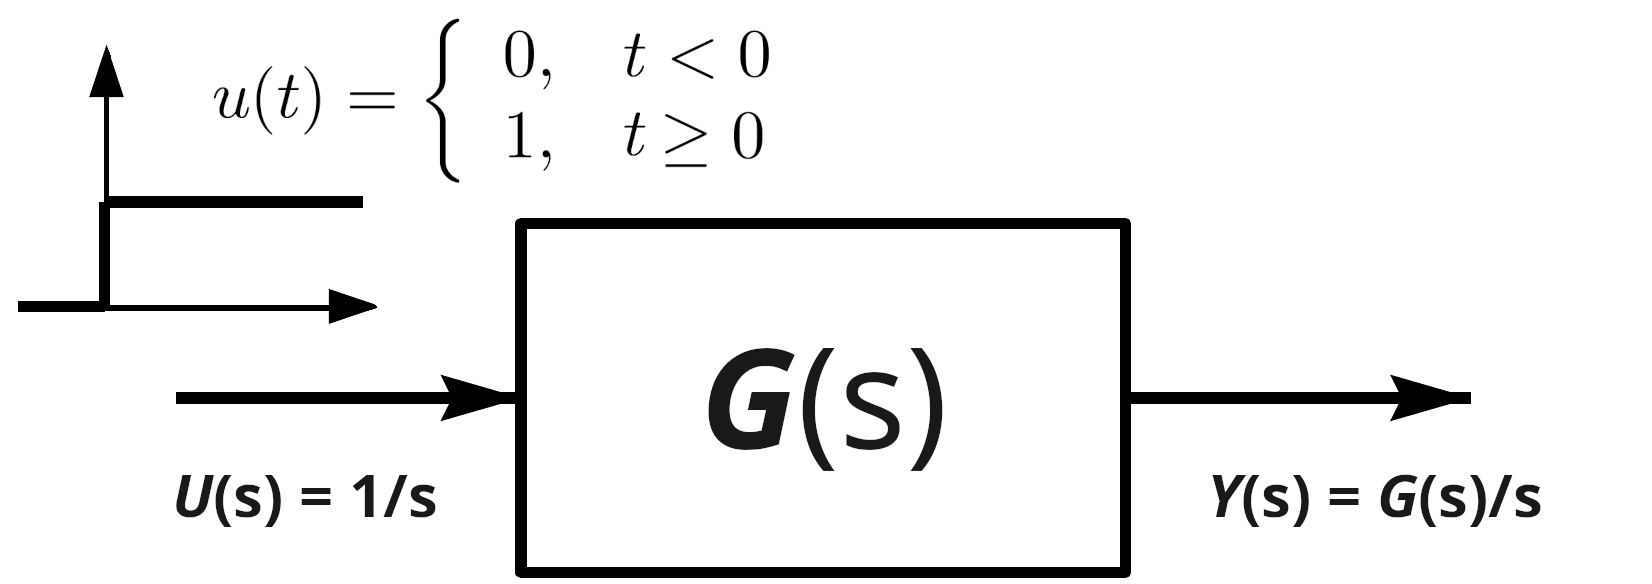
\includegraphics[width = 0.5\linewidth]{img/state-space-models/unit-step-response.png}
    \caption{Resposta do sistema ao degrau unitário.}
    \label{fig:unit-step-response}
\end{figure}

{
\mdfsetup{linewidth=2pt}

\begin{mdframed}
    \begin{itemize}
    \item[$\blacktriangle$] \underline{Valor final da resposta} ao escalão unitário:
        
        \vspace{-1em}
        $$
            \lim_{t \to +\infty} y(t) = \lim_{s \to 0} sY(s) = \lim_{s \to 0} s\frac{G(s)}{s} = G(0)
        $$
        
    \vspace{-0.5em}
    \item[$\blacktriangle$] \underline{Valor inicial da resposta} ao escalão:
        
        \vspace{-1em}
        $$
            \lim_{t \to 0} y(t) = \lim_{s \to +\infty} sY(s) = \lim_{s \to +\infty} s\frac{G(s)}{s} = \lim_{s \to +\infty} G(s)
        $$
        
    \vspace{-0.5em}
    \item[$\blacktriangle$] \underline{Valor inicial da derivada da resposta} ao escalão unitário:
        
        \vspace{-1em}
        $$
            \lim_{t \to 0} \dot{y}(t) = \lim_{s \to +\infty} s\, (sY(s)) = \lim_{s \to +\infty} s^2\frac{G(s)}{s} = \lim_{s \to +\infty} sG(s)
        $$

    \vspace{-0.5em}
    \item[$\blacktriangle$] \underline{Valor final da derivada da resposta} ao escalão unitário:
        
        \vspace{-1em}
        $$
            \lim_{t \to +\infty} \dot{y}(t) = \lim_{s \to 0} s\, (sY(s)) = \lim_{s \to 0} s^2\frac{G(s)}{s} = \lim_{s \to 0} s G(s)
        $$
    \end{itemize}
\end{mdframed}
}

\vspace{-1em}
\paragraph[1.2.2.1 Excesso de pólos-zeros]{$\pmb{\star}$ Excesso de polos-zeros (resposta ao escalão unitário)}\mbox{}\\
\begin{center}%
    \begin{tabular}{c c}%
        \begin{minipage}{0.425\linewidth}%
            \vspace{-1em}
            \begin{mdframed}
                $$
                    \lim_{t \to 0} y(t) = \lim_{s \to +\infty} G(s)
                $$
            \end{mdframed}
        \end{minipage}%
        &%
        \begin{minipage}{0.425\linewidth}%
            \vspace{-1em}
            \begin{mdframed}
                $$
                    \lim_{t \to 0} \dot{y}(t) = \lim_{s \to +\infty} sG(s)
                $$
            \end{mdframed}
        \end{minipage}%
    \end{tabular}%
\end{center}%

{\setlength{\tabcolsep}{16pt}
\begin{center}
    \begin{tabular}{p{0.4\textwidth} | p{0.4\textwidth}}
        \centerline{\underline{$\#\textbf{pólos} > \#\textbf{zeros}$}} & \centerline{\underline{$\#\textbf{pólos} > \#\textbf{zeros}+1$}} \\[-14pt]
        Resposta ao escalão contínua & Derivada da resposta contínua \\[4pt]
        \centerline{\underline{$\#\textbf{pólos} = \#\textbf{zeros}$}} & \centerline{\underline{$\#\textbf{pólos} = \#\textbf{zeros}+1$}} \\[-14pt]
        Resposta descontínua, com salto finito & Derivada da resposta descontínua, mas finita \\[4pt]
        \centerline{\underline{$\#\textbf{pólos} < \#\textbf{zeros}$}} & \centerline{\underline{$\#\textbf{pólos} < \#\textbf{zeros}+1$}} \\[-14pt]
        Resposta descontínua, com salto infinito & Derivada da resposta descont.,  infinita \\
        \bottomrule
    \end{tabular}
\end{center}
}

\renewcommand*{\thefootnote}{\fnsymbol{footnote}}
\footnotetext[4]{\underline{\textbf{Nota:}} caso um dos zeros se encontre no SPD, então temos um sistema de \underline{fase não mínima}.}
\renewcommand*{\thefootnote}{\arabic{footnote}}

%//==============================--C--==============================//%
\subsubsection[1.2.3 Sistemas de 2\textordfeminine{} ordem (sem zeros)]{$\pmb{\rightarrow}$ Sistemas de 2\textordfeminine{} ordem (sem zeros)}

$$
    G(j\omega) = \frac{\omega_n^2}{s^2 + 2\zeta\omega_ns + \omega_n^2}
$$

\begin{mdframed}
    \noindent $\zeta$ - Determina a forma da resposta.\\
    \noindent $\omega_n$ - Determina a escala de tempo.\\ 
    \noindent Quando maior for $\omega_n$ maior é a largura de banda e mais rápido é o sistema.
\end{mdframed}

\vspace{-0.5em}
\begin{figure}[H]
    \label{fig:second-order-system-step-response}
    \begin{subfigure}[b]{0.5\linewidth}
        \centering
        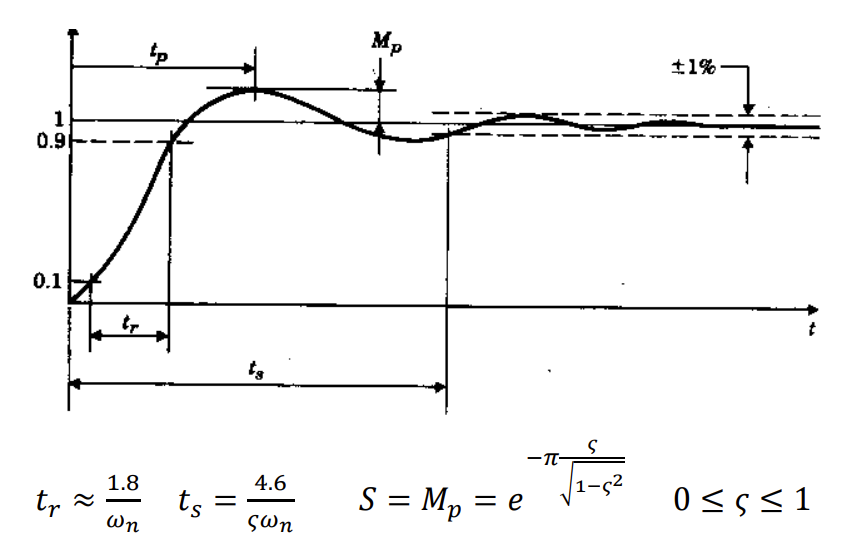
\includegraphics[width=0.8\linewidth]{img/state-space-models/second-order-system-step-response.png}
        \label{fig:second-order-step-response} 
    \end{subfigure}
    \begin{subfigure}[b]{0.5\linewidth}
        \centering
        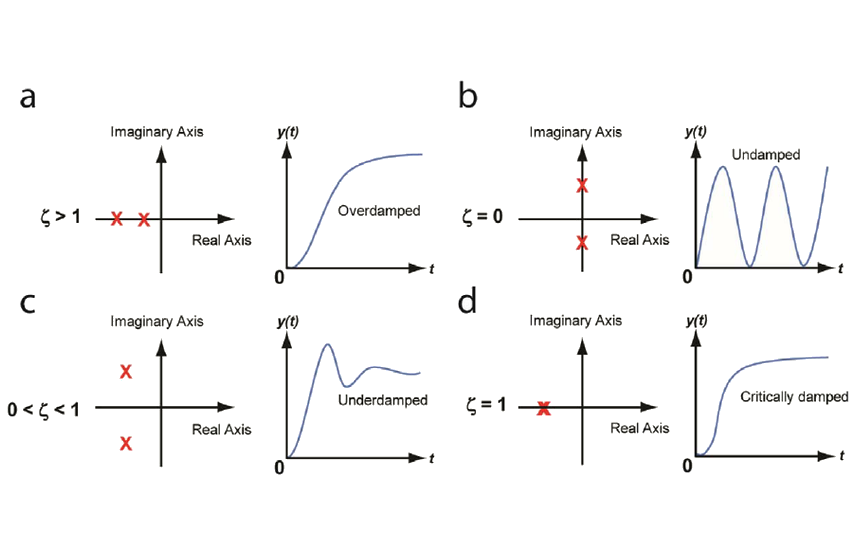
\includegraphics[width=0.85\linewidth]{img/state-space-models/step-response-second-order-system.png} 
        \label{fig:second-order-dif-cases} 
    \end{subfigure}
    \begin{minipage}{1\linewidth}
        \vspace{-1.5em}
        \caption{Tipos de resposta de sistemas de segunda ordem sem zeros ($\star$ resposta ao escalão unitário).}
    \end{minipage}
\end{figure}

%//==============================--D--==============================//%
\subsubsection[1.2.4 Diagramas de Bode]{$\pmb{\rightarrow}$ Diagramas de Bode}

``The most useful technique for hand plotting was developed by H. W. Bode at Bell Laboratories between 1932 and 1942. The idea in Bode's method is to plot magnitude curves using a logarithmic scale and phase curves using a linear scale. This strategy allows us to plot a high-order $G(j\omega)$ by simply adding the separate terms graphically.
$$
    \frac{\bar{s}_1 \bar{s}_2}{\bar{s}_3 \bar{s}_4 \bar{s}_5} = \frac{r_1 e^{j\theta_1} r_2 e^{j\theta_2}}{r_3 e^{j\theta_3} r_4 e^{j\theta_4} r_5 e^{j\theta_5}} =
    \left( \frac{r_1 r_2}{r_3 r_4 r_5} \right) e^{j(\theta_1 + \theta_2 - \theta_3 - \theta_4 - \theta_5)}
$$
phases of the individual terms are added directly to obtain the phase of the composite expression, $G(j\omega)$. Furthermore, because
$$
    \vert G(j\omega) \vert = \frac{r_1 r_2}{r_3 r_4 r_5}
$$
it follows that
$$
    \log_{10}\vert G(j\omega) \vert = \log_{10}(r_1) + \log_{10}(r_2) - \log_{10}(r_3) - \log_{10}(r_4) - \log_{10}(r_5).\text{''\cite{FranklinPowell2015}}
$$

\begin{figure}[H]
    \centering
    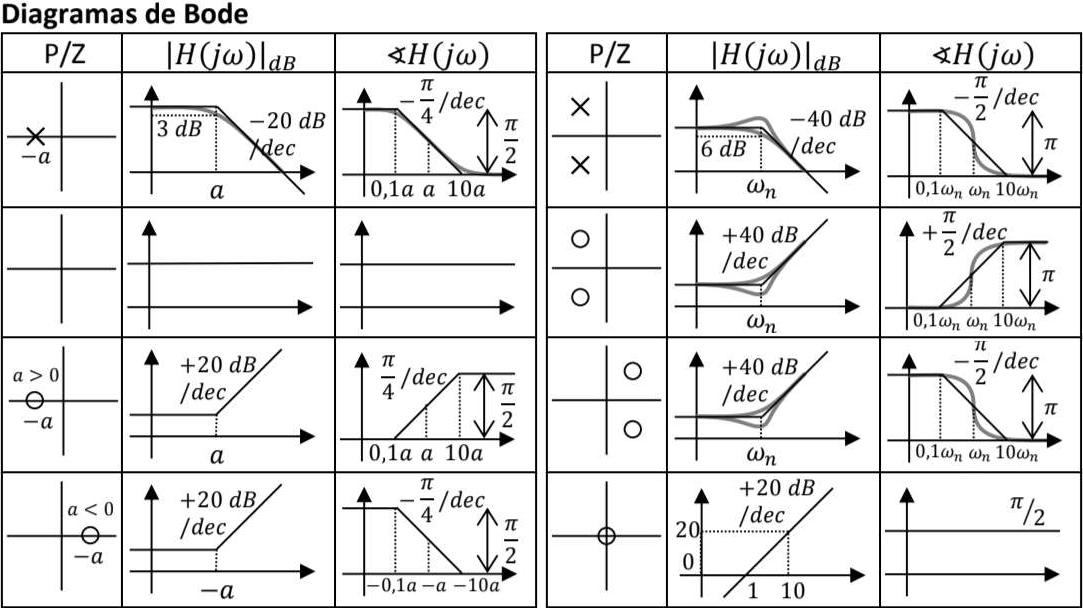
\includegraphics[width = 0.7\linewidth]{img/state-space-models/bode.png}
    \caption{Resposta assimtótica---resposta em diagramas de Bode.}
    \label{fig:bode}
\end{figure}

%Adoro-te cutie 
%cutie :3 adoro-te
%//==============================--@--==============================//%

    \clearpage
    \section{2. Linearização de Sistemas Não Lineares}
        %//==============================--@--==============================//%
\label{sec:linearisation}

\noindent A aproximação linear de uma função é o \underline{polinómio de Taylor de primeira ordem} em torno do ponto de interesse. Em sistemas dinâmicos, é um método que permite (\hyperref[def:equilibrium-point]{possivelmente}) aferir a estabilidade local de pontos de equilíbrio de sistemas não lineares.

{
\mdfsetup{linewidth=2pt}

\begin{mdframed}
    \noindent Seja $\pmb{\dot{x}} = f(\pmb{x})$, não linear. A equação geral para a linearização de uma função multivariável $f(\pmb{x})$ num ponto $\pmb{p}$ é:
    \vspace{-0.5em}
    $$
        f(\pmb{x}) \approx f(\pmb{p}) + \left.D f\right|_{\pmb{p}} \cdot (\pmb{x} - \pmb{p})
    $$
    
    \noindent onde $\pmb{x}$ é o vetor de variáveis e $\pmb{p}$ o ponto de interesse para a linearização.
\end{mdframed}
}

\begin{quote}
    \noindent ``A good place to start analyzing the nonlinear system 
    $$
        \pmb{\dot{x}} = f(\pmb{x}) 
    $$
    is to determine its \underline{equilibrium points} and describe its behavior near [this points]. (...) the local behavior of the nonlinear system near a hyperbolic equilibrium point $\pmb{p}$ is qualitatively determined by the behavior of the linear system
    $$
        \pmb{\dot{x}} = \pmb{A}\,\pmb{x},
    $$
    with the matrix $\pmb{A} = Df(\pmb{p})$, near the origin. 
    
    The linear function $\pmb{A}\, \pmb{x} = Df(\pmb{p})\, \pmb{x}$ is called the \textit{linear part} of $f$ at $\pmb{p}$.''\cite{Perko2013}
\end{quote}

\begin{theo}[\underline{Def.:} Ponto de equilíbrio (ou ponto critico)\cite{Perko2013}]{def:equilibrium-point}\label{def:equilibrium-point}
    A point $\pmb{p} \in \mathbb{R}^n$ is called an \textit{equilibrium point} or \textit{critical point} of $\pmb{\dot{x}} = f(\pmb{x})$ if $f(\pmb{p}) = 0$. An equilibrium point $\pmb{p}$ is called a \textit{hyperbolic equilibrium point} of $\pmb{\dot{x}} = f(\pmb{x})$ if none of the eigenvalues of the matrix $Df(\pmb{p})$ have zero real part. The linear system $\pmb{\dot{x}} = \pmb{A}\,\pmb{x}$ with the matrix $\pmb{A} = D f(\pmb{p})$ is called the \textit{linearization} of $\pmb{\dot{x}} = f(\pmb{x})$ at $\pmb{p}$.
\end{theo}

\begin{quote}
    ``The Hartman-Grobman Theorem is another very important result in the local qualitative theory of ordinary differential equations. The theorem shows that near a hyperbolic equilibrium point $\pmb{p}$, the nonlinear system
    $$
        \pmb{\dot{x}} = f(\pmb{x})
    $$
    has the same qualitative structure as the linear system
    $$
        \pmb{\dot{x}} = \pmb{A}\,\pmb{x}
    $$    
    with $\pmb{A} = Df(\pmb{p})$. Throughout this section we shall assume that the equilibrium point \underline{$\pmb{p}$ has been translated to the origin}.''\cite{Perko2013}
\end{quote}

\begin{theo}[\underline{Definition 1} \cite{Perko2013}]{def:lin-theorem}\label{def:lin-theorem}
    Two autonomous systems of differential equations such as $\pmb{\dot{x}} = f(\pmb{x})$ and $\pmb{\dot{x}} = \pmb{A}\,\pmb{x}$ are said to be \textit{topologically equivalent} in a neighborhood of the origin or to have the \textit{same qualitative structure near the origin} if there is a homeomorphism $H$ mapping an open set $U$ containing the origin onto an open set $V$ containing the origin which maps trajectories of $\pmb{\dot{x}} = f(\pmb{x})$ in $U$ onto trajectories of $\pmb{\dot{x}} = \pmb{A}\,\pmb{x}$ in $V$ and preserves their orientation by time in the sense that if a trajectory is directed from $\pmb{p_1}$ to $\pmb{p_2}$ in $U$, then its image is directed from $H(\pmb{p_1})$ to $H(\pmb{p_2})$ in $V$. If the homeomorphism $H$ preserves the parameterization by time, then the systems $\pmb{\dot{x}} = f(\pmb{x})$ and $\pmb{\dot{x}} = \pmb{A}\,\pmb{x}$ are said to be \textit{topologically conjugate} in a neighborhood of the origin.
\end{theo}

\begin{theo}[\underline{Teo.:} Teorema da Linearização (Hartman-Grobman)\cite{Perko2013}]{teo:lin-theorem}\label{teo:lin-theorem}
     Let $E$ be an open subset of $\mathbb{R}^n$ containing the origin, let $f \in C^1(E)$, and let $\phi_t$ be the flow of the nonlinear system $\pmb{\dot{x}} = f(\pmb{x})$. Suppose that $f(\pmb{p}) = 0$ and that the matrix $\pmb{A} = Df(\pmb{p})$ has no eigenvalue with zero real part. Then there exists a homeomorphism $H$ of an open set $U$ containing the origin onto an open set $V$ containing the origin such that for each $\pmb{p}\in U$, there is an open interval $I_0 \subset \mathbb{R}$ containing zero such that for all $\pmb{p} \in U$ and $t \in I_0$ 
     $$
        H \circ \phi_t(\pmb{p}) = e^{\pmb{A}t} H(\pmb{p}); 
     $$
     i.e., $H$ maps trajectories of $\pmb{\dot{x}} = f(\pmb{x})$ near the origin onto trajectories of $\pmb{\dot{x}} = \pmb{A}\,\pmb{x}$ near the origin and preserves the parameterization by time.
\end{theo}

{
\mdfsetup{linewidth=2pt}

\begin{mdframed}
    \noindent $\pmb{\rightarrow}$ \textbf{\textit{Procedimentos}:}
    \begin{itemize}
        \item[$\blacktriangle$] \hyperref[def:equilibrium-point]{Calcular os pontos de equilíbrio}

        \item[$\blacktriangle$] \hyperref[def:equilibrium-point]{Calcular a Matriz Jacobiana e aferir que pontos de equilíbrio são hiperbólicos}. Invocar o \hyperref[teo:lin-theorem]{Teorema da Linearização} e justificar que lineariza- ções representam qualitativamente o comportamento do sistema não linear na vizinhança dos pontos de equilíbrio respetivos. 

        \item[$\blacktriangle$] Traçar qualitativamente o retrato de fase para os \hyperref[def:equilibrium-point]{pontos de equilíbrio hiperbólicos} (\textit{vide} \hyperref[subsec:phase-plane-analysis]{Phase Plane Analysis}).
    \end{itemize}

    \noindent $\pmb{\rightarrow}$ \textbf{\textit{Nota}:}
    
    \noindent Para matrizes $\pmb{A}$ $[2 \times 2]$, os valores próprios são dados por:
    $$
        \lambda_{1,2} = \frac{1}{2}\text{tr}[\pmb{A}] \pm \frac{1}{2}\sqrt{\left(\text{tr}[\pmb{A}] \right)^2 - 4\det[\pmb{A}]}
    $$
\end{mdframed}
}
%//==============================--@--==============================//%
        {\pagestyle{empty}
        \includepdf[pages=1,pagecommand={\subsection[2.1 Phase Plane Analysis]{}\label{subsec:phase-plane-analysis}}]{pdfs/Phase-Plane-Analysis}
        \includepdf[pages=2-,pagecommand={}]{pdfs/Phase-Plane-Analysis}}
        \pagestyle{fancy}

    \clearpage
    \section{3. Modelação Física}
    \def\equalfootnote{\mathrel{\ensurestackMath{\stackon[1pt]{=}{\footnotemark[0]}}}}
%//==============================--@--==============================//%
\label{sec:mechanics}
\subsection[3.1 Sistemas Mecânicos de Translação]{$\rightarrow$ Sistemas Mecânicos de Translação}
\label{sec:mechanics-translation}

``The cornerstone for obtaining a mathematical model, or the dynamic equations, for any mechanical system is Newton's law
$$
    \boxed{F = \frac{dp}{dt} = \frac{d}{dt} (m v) \equalfootnote ma}
$$
\noindent where:
\begin{itemize}
    \item $F$ = the vector sum of all forces applied to each body in a system, newtons (N),
    \item $p$ = linear momentum/translational momentum (kg ms$^{-1}$),
    \item $v$ = velocity (ms$^{-1}$), the directional speed of an object in motion as an indication of its rate of change in position as observed from a particular frame of reference,
    \item $a$ = the vector acceleration of each body with respect to an inertial reference frame (that is, one that is neither accelerating nor rotating with respect to the stars); often called inertial acceleration, ms$^{-2}$,
    \item $m$ = mass of the body, kg.''\cite{FranklinPowell2015}
\end{itemize}

\footnotetext[0]{Para uma massa invariante no tempo, ou aproximadamente constante.}

\phantomsection\addcontentsline{toc}{subsubsection}{3.1.1 Relações fundamentais baseadas em princípios físicos}
\renewcommand*{\thefootnote}{\fnsymbol{footnote}}
\begin{theo}[\underline{Molas Elásticas}]{def:Molas Elásticas}\label{def:MolasElásticas}
Quando uma mola é comprimida ou esticada, reage com uma força que se opõe à compressão (ou à extensão). Força desta que, para molas lineares, é dada por:
$$
    f = -kx
$$
Onde $k$ é a constante de Hooke [N/m].
\end{theo}

\begin{theo}[\underline{Atrito Viscoso}]{def:Atrito Viscoso}\label{def:AtritoViscoso}
Elemento que dissipa energia. Quando existe uma diferença de velocidade entre dois corpos o atrito corresponde a uma força que contraria o movimento. No caso linear, o atrito é dado por:
$$
    f = -\beta\dot{x}\ = -\beta v 
$$
\end{theo}

\mdfsetup{linewidth=2pt}
\begin{mdframed}
\textbf{Nota} $\rightarrow$ \textbf{Atrito estático} 

\noindent 
``Static friction is also known as stiction and models the fact that in some cases the friction
force is larger in magnitude for zero velocity than for a non-zero velocity. According to
the stiction model the system sticks if the velocity is zero and $|F_t | < F_s$, and it breaks
away if $|F_t | = F_s$ where $F_s > F_a$''\cite{Egeland2002}
\end{mdframed}

%//==============================--@--==============================//%
\clearpage
\subsection[3.2 Sistemas Mecânicos de Rotação]{$\rightarrow$ Sistemas Mecânicos de Rotação}
\label{sec:mechanics-rotation}

O \underline{Momento de Inércia} é o análogo da massa para a rotação. Quando um corpo em rotação com um \underline{Momento de Inércia} $J$ $[$Nms$^{2}]$ é atuado por um \underline{Binário} $T$ $[$Nm$]$, adquire aceleração angular dada por
$$
    \boxed{J\ddot{\theta} = T}
$$


\begin{theo}[\underline{Molas Elásticas}]{def:Mola Elástica de Rota}\label{def:MolaElasticaRota}
Quando a mola é desviada um ângulo $\theta$  em relação à posição de repouso, reage
com um binário que se opõe ao movimento, dada para molas lineares por:
$$
    T = -K\dot{\theta}\ 
$$
Onde $k$ é a "constante da mola" [Nm/rads$^{-1}$].
\end{theo}

\begin{theo}[\underline{Atrito Viscoso}]{def:Atrito Viscoso Rotação}\label{def:AtritoViscosoRotação}
Elemento que dissipa energia. Quando existe uma diferença de velocidade de rotação entre dois corpos o atrito corresponde a uma binário que contraria o movimento e que depende da velocidade angular. No caso linear, o atrito é dado por:
$$
    T = -\beta\dot{\theta}\ = -\beta \omega
$$
\end{theo}

\begin{theo}[\underline{Caixa de desmultiplicação}]{def:Caixa D}\label{def:Caixa D}
Uma caixa de desmultiplicação transforma o binário e a velocidade angular de acordo com as seguintes relações:
$$
    \omega_1 = \frac{1}{a}\omega_1\qquad
    T_1 = aT_2\qquad
    T_1 \omega_1 = T_2 \omega_2
$$

Onde $a = \frac{\omega_1}{\omega_2}$ é o inverso da razão de desmultiplicação da caixa.
\end{theo}




\begin{theo}[\underline{Transformação da rotação em translação}]{def:rotation-to-translation}\label{def:rotation-to-translation}
Assumindo que não existe escorregamento, nem perdas energéticas, temos
$$
    v = \omega r,\qquad F = \frac{1}{r} T
$$
\vspace{-1em}
\begin{figure}[H]
    \centering
    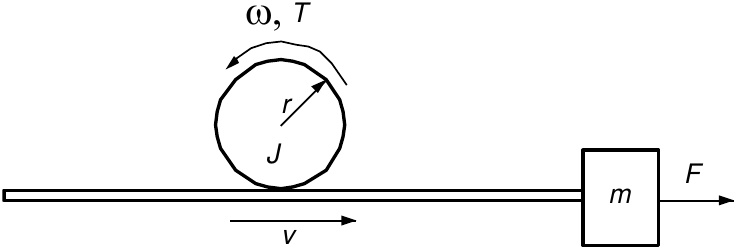
\includegraphics[width = 0.6\linewidth]{img/mechanics/convertion.png}
    \label{fig:convertion}
\end{figure}
\end{theo}

% \begin{figure}[H]
%     \centering
%     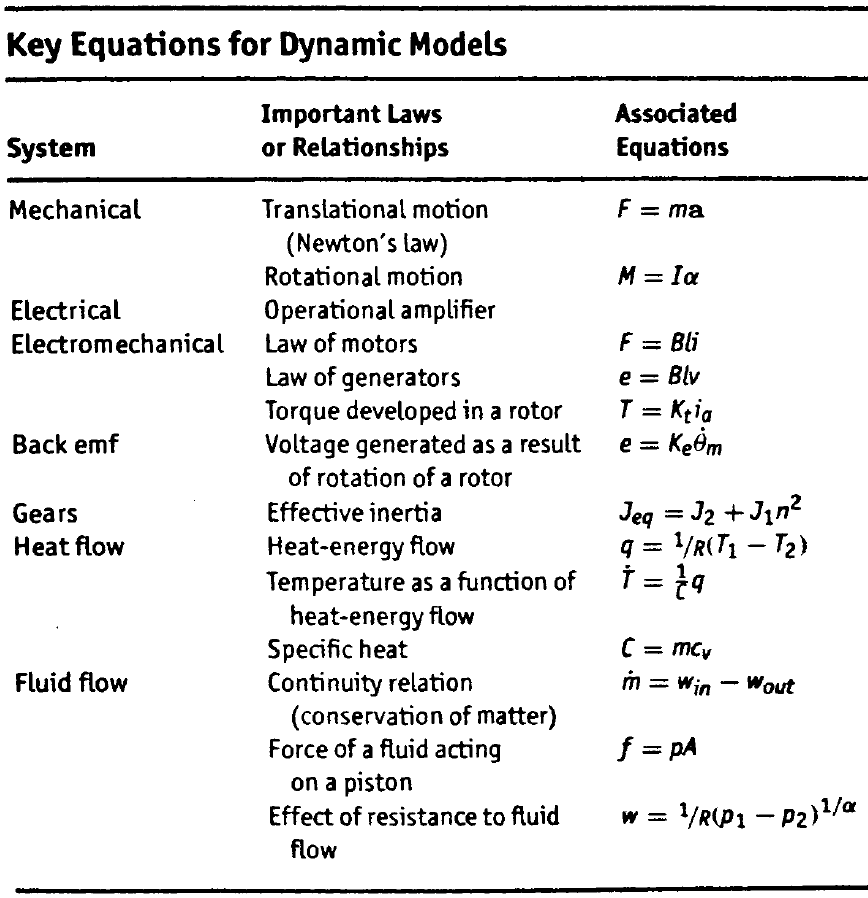
\includegraphics[width = 0.7\linewidth]{img/mechanics/key-equations.png}
%     \caption{Equações chave. \textbf{\underline{Nota:}} $M = I \alpha \iff J\ddot{\theta} = T$}
%     \label{fig:key-equations}
% \end{figure}
%//==============================--@--==============================//%
\newpage
\subsubsection[3.2.2 Motor Corrente Contínua]{$\rightarrow$ Motor de Corrente Contínua}
\mdfsetup{linewidth=2pt}
\begin{mdframed}
\textbf{Modelo do servomotor CC de íman permanente:}

\noindent\underline{Binário do motor}: Para um fluxo constante

\noindent \hspace*{1.5 em}\raisebox{0.2 em}{$\drsh$} $T(t) = K_T\, i(t)$

\vspace{0.5em}
\noindent\underline{Tensão aos terminais do rotor}: 

\noindent \hspace*{1.5 em}\raisebox{0.2 em}{$\drsh$} $e = K_e\, \omega$
%adoro-te :3 miminhooooooooooooooooooooooooooooooooooooooos

% cutie :3 -><- aaaaaaadoro-te
\end{mdframed}
\paragraph[3.2.2.1 Problema 1]{$\pmb{\star}$ Escreva as equações que modelam o sistema na forma de um modelo de estado (sistema
de equações diferenciais de 1ª ordem)}\mbox{}\\
\begin{figure}[H]
    \centering
    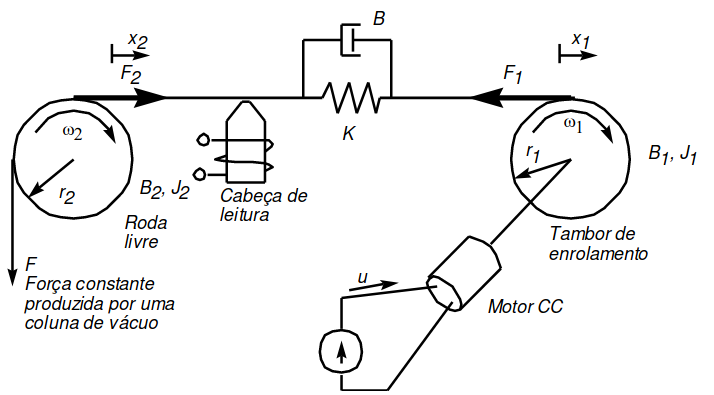
\includegraphics[width = 0.6\linewidth]{img/mechanics/motor-cc-P16.png}
    \caption{P16 retirado da coletânea de exercícios.}
    \label{fig:motor-cc-P16}
\end{figure}

\noindent\underline{T. de Enrolamento}: de acordo com as equações subjacentes à mecânica de rotação

\noindent \hspace*{1.5 em}\raisebox{0.2 em}{$\drsh$} $J_1 \dot{\omega_1} = - F_1 r_1 - \beta_1 \omega_1 + T_{cc}$

\vspace{0.5em}
\noindent\underline{Roda Livre}: novamente, de acordo com as equações subjacentes à mecânica de rotação 

\noindent \hspace*{1.5 em}\raisebox{0.2 em}{$\drsh$} $J_1 \dot{\omega_2} = (F_2 - F) r_2 - \beta_2 \omega_2$

\vspace{0.5em}
\noindent\underline{Fita}: (\textit{vide} \hyperref[def:MolasElásticas]{secção das molas elásticas})

\noindent \hspace*{1.5 em}\raisebox{0.2 em}{$\drsh$} $
                \begin{cases}
                    F_1 = K(x_1 - x_2) + \beta(\dot{x_1} - \dot{x_2})\\
                    F_2 = -K(x_2 - x_1) - \beta(\dot{x_2} - \dot{x_1})\\
                \end{cases}
$

\vspace{0.5em}
\noindent\underline{Motor CC}: $T_{cc}$ é o binário exercido pelo motor CC no Tambor de Enrolamento

\noindent \hspace*{1.5 em}\raisebox{0.2 em}{$\drsh$} $T_{cc} = K_T\, u$

\vspace{0.5em}
\noindent\underline{Variáveis do referencial}: a velocidade linear de um ponto da periferia de uma roda é o produto do raio da roda pela velocidade angular

\noindent \hspace*{1.5 em}\raisebox{0.2 em}{$\drsh$} $
                \begin{cases}
                    \dot{x_1} = \omega_1 r_1\\
                    \dot{x_2} = \omega_2 r_2\\
                \end{cases}
$

%//==============================--@--==============================//%
\clearpage
\paragraph[3.2.2.2 Problema 2]{$\pmb{\star}$ Escreva as equações que modelam o sistema e um modelo de estado na forma de um sistema de
equações diferenciais de 1ª ordem.}\mbox{}\\
\begin{figure}[H]
    \centering
    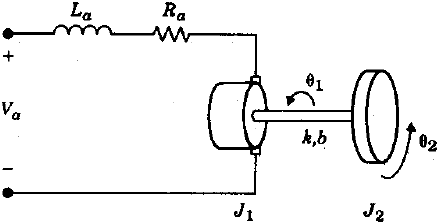
\includegraphics[width = 0.45\linewidth]{img/mechanics/motor-cc-P18.png}
    \caption{P18 retirado da coletânea de exercícios. Motor elétrico que reboca uma carga com um modo dominante de vibração.}
    \label{fig:motor-cc-P18}
\end{figure}

\noindent \underline{Motor:} por aplicação da Lei das Malhas (KVL)

\noindent \hspace*{1.5 em}\raisebox{0.2 em}{$\drsh$} \textbf{KVL}: $ L_a \dfrac{d i_a}{dt} + i_a R_a + e_a - V_A = 0 \iff \dfrac{d i_a}{dt} = -\dfrac{K_e}{L_a} \dot{\theta}_1 - \dfrac{R_a}{L_a} i_a + V_A$

\vspace{0.5em}
\noindent \underline{Veio:} com as equações subjacentes à mecânica de rotação

\noindent \hspace*{1.5 em}\raisebox{0.2 em}{$\drsh$} $J_1 \ddot{\theta}_1 = -K(\theta_1 - \theta_2) -\beta(\dot{\theta}_1 - \dot{\theta}_2) + T_{cc}$

\vspace{0.5em}
\noindent\underline{Motor CC}: $T_{cc}$ é o binário exercido pelo motor CC no veio

\noindent \hspace*{1.5 em}\raisebox{0.2 em}{$\drsh$} $T_{cc} = K_T\, i_a$

\vspace{0.5em}
\noindent \underline{Carga:} de acordo com as equações subjacentes à mecânica de rotação

\noindent \hspace*{1.5 em}\raisebox{0.2 em}{$\drsh$} $J_2 \ddot{\theta}_2 = -K(\theta_2 - \theta_1) -\beta(\dot{\theta}_2 - \dot{\theta}_1)$

\vspace{0.5em}
\noindent Definem-se então os estados: $\pmb{x} = \begin{bmatrix} \theta_2 & \dot{\theta}_2 & \theta_1 & \dot{\theta}_1 & i_a\end{bmatrix}^T$

$$
    \therefore \dot{\pmb{x}} = 
    \begin{bmatrix} 
        0 & 1 & 0 & 0 & 0\\[4pt]
        -\frac{K}{J_2} & -\frac{\beta}{J_2} & \frac{K}{J_2} & \frac{\beta}{J_2} & 0\\[4pt]
        0 & 0 & 0 & 1 & 0\\[4pt]
        \frac{K}{J_1} & \frac{\beta}{J_1} & -\frac{K}{J_1} & -\frac{\beta}{J_1} & K_T\\[4pt]
        0 & 0 & 0 & -\frac{K_e}{L_a} & -\frac{R_a}{L_a}
    \end{bmatrix}
    \pmb{x} +
    \begin{bmatrix} 
        0\\
        0\\
        0\\
        0\\
        -\frac{1}{L_a}
    \end{bmatrix}
    V_A
$$

%//==============================--@--==============================//%
\clearpage
\paragraph[3.2.2.3 Problema 3]{$\pmb{\star}$ Defina um estado apropriado com a menor dimensão possível e escreva as respetivas equações de estado na forma matricial. }\mbox{}\\
\begin{figure}[H]
    \centering
    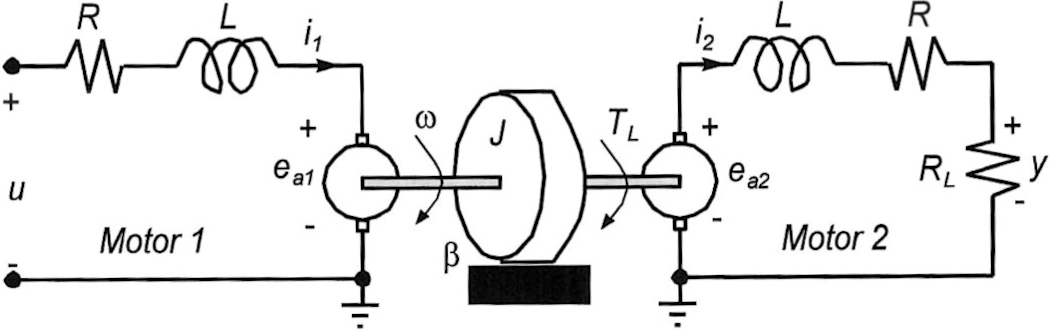
\includegraphics[width = 0.6\linewidth]{img/mechanics/motor-cc-exame2021.png}
    \caption{Circuito eletromecânico equivalente de dois motores de corrente contínua de íman permanente, que têm os veios ligados solidariamente. $T_L = K_T\, i_1$ e $e_{ai} = K_{ei}\, \omega$}
    \label{fig:motor-cc-exame20/21}
\end{figure}

\noindent \underline{Motor 1:} por aplicação da Lei das Malhas (KVL)

\noindent \hspace*{1.5 em}\raisebox{0.2 em}{$\drsh$} \textbf{KVL}: $i_1 R + L \dfrac{d i_1}{dt} + e_{a1} - u = 0 \iff \dfrac{d i_1}{dt} = - \dfrac{R}{L} i_1 - \dfrac{K_{e1}}{L} \omega + \dfrac{1}{L}u$

\vspace{0.5em}
\noindent \underline{Motor 2:} por aplicação, novamente, da Lei das Malhas (KVL)

\noindent \hspace*{1.5 em}\raisebox{0.2 em}{$\drsh$} \textbf{KVL}: $L \dfrac{d i_2}{dt} + i_2 R + i_2 R_L - e_{a2} = 0 \iff \dfrac{d i_2}{dt} = \dfrac{K_{e2}}{L}\omega - \left(\dfrac{R+R_L}{L}\right) i_2$

\vspace{0.5em}
\noindent \underline{Roda:} de acordo com as equações subjacentes à mecânica de rotação

\noindent \hspace*{1.5 em}\raisebox{0.2 em}{$\drsh$} $J \dot{\omega} = T_L - \beta \omega \iff \dot{\omega} = -\dfrac{\beta}{J}\omega + \dfrac{K_T}{J} i_1$

\vspace{0.5em}
\noindent Definem-se então os estados: $\pmb{x} = \begin{bmatrix} \omega & i_1 & i_2 \end{bmatrix}^T$

$$
    \therefore \dot{\pmb{x}} = 
    \begin{bmatrix} 
        -\frac{\beta}{J} & \frac{K_T}{J} & 0\\[5pt]
        -\frac{K_{e1}}{L} & -\frac{R}{L} & 0\\[5pt]
        \frac{K_{e2}}{L} & 0 & \frac{K_T}{J}
    \end{bmatrix}
    \pmb{x} +
    \begin{bmatrix} 
        0\\[5pt]
        \frac{1}{L}\\[5pt]
        0
    \end{bmatrix}
    u,\qquad y = 
    \begin{bmatrix}
        0 & 0 & R_L
    \end{bmatrix}
    \pmb{x}
$$

%//==============================--@--==============================//%
\clearpage
\subsection[3.2 Sistemas baseados em Mecânica Lagrangiana]{$\rightarrow$ Sistemas baseados em Mecânica Lagrangiana}
\label{sec:mechanics-lagrangian}

\phantomsection\addcontentsline{toc}{subsubsection}{3.2.1 Princípio de Hamilton}
\renewcommand*{\thefootnote}{\fnsymbol{footnote}}
\begin{theo}[\underline{Princípio de Hamilton} \cite{Maia2000}]{def:principio-hamilton}\label{def:principio-hamilton}
    De todo o conjunto de configurações admissíveis que um sistema pode assumir ao evoluir de uma configuração $1$ no instante $t_1$ para uma configuração $2$ no instante $t_2$, aquela que satisfaz as condições de equilíbrio dinâmico em cada instante é a que torna estacionário (mínimo) o integral da Lagrangiana\footnotemark[2] do sistema durante esse intervalo de tempo.
\end{theo}

\noindent ``Matematicamente, a condição de equilíbrio dinâmico corresponde a
$$
    \delta I = \delta \int_{t_1}^{t_2} (T-U) \, dt = \delta \int_{t_1}^{t_2} L \, dt = 0 
$$
em que $\delta$ representa a primeira variação de $I$. Não se trata de uma minimização clássica de uma função em relação a uma ou mais variáveis, pois das várias funções associadas às várias trajectórias possíveis, expressas pelo integral $I$, à sua minimização corresponde também uma função, que é a trajectória de equilíbrio. $I$ não é uma função, mas antes uma função de funções, que se designa por funcional.''\cite{Maia2000}
\noindent{\begin{center}\rule{8cm}{1pt} \end{center}} 

\footnotetext[2]{``\underline{\textbf{Note-se}} que a Lagrangiana, $L=T-V$, é uma medida do balanço entre a energia cinética e a energia potencial. Compreende-se, pois, que a integração no tempo dessa medida corresponde a uma situação de equilíbrio dinâmico.''\cite{Maia2000}}
\renewcommand*{\thefootnote}{\arabic{footnote}}

\noindent O princípio de Hamilton pode ser encarado como a integração no tempo do princípio dos trabalhos virtuais em dinâmica.

\begin{mdframed}
$$
    \therefore \int_{t_1}^{t_2} (\delta L + \overline{\delta W}_{\text{nc}}) \, dt = 0,\quad \delta r_i (t_1) = \delta r_i (t_2) = 0,\quad i = 1,\dots,N  
$$
\end{mdframed}
em que $\overline{\delta W}_{\text{nc}}$ representa o trabalho virtual das forças não-conservativas. Esta expres- são traduz o \underline{\textit{princípio de Hamilton generalizado}}\cite{Maia2000}.

\subsubsection[3.2.2 Equações de Euler-Lagrange]{$\rightarrow$ Equações de Euler-Lagrange}

É possível deduzir de uma forma muitíssimo elegante as equações de Lagrange através do princípio de Hamilton.

\begin{theo}[\underline{Equações de Euler-Lagrange} \cite{Maia2000}]{def:euler-lagrange}\label{def:euler-lagrange}
$$
    \frac{d}{dt}\left( \frac{\partial L}{\partial \dot{q}_k} \right) - \frac{\partial L}{\partial q_k} = Q_k,\quad k = 1,2,\dots,n
$$

\noindent em que $Q_k$ são as forças generalizadas não-conservativas.
\end{theo}

 \noindent ``Note-se que basta conhecer-se a Lagrangiana do sistema, que é um escalar, e as forças externas aplicadas, para---de uma forma directa---se obterem as equações de equilíbrio dinâmico. Naturalmente, a expressão indica que se obtêm $n$ equações, dado que o sistema tem $n$ graus de liberdade. ''\cite{Maia2000}

Se não existirem forças externas aplicadas, o sistema encontrar-se-á em movimento livre e a equação simplifica-se:
$$
    \frac{d}{dt}\left( \frac{\partial L}{\partial \dot{q}_k} \right) - \frac{\partial L}{\partial q_k} = 0,\quad k = 1,2,\dots,n
$$

%//==============================--@--==============================//%
\subsection[3.3 Sistemas Térmicos]{$\rightarrow$ Sistemas Térmicos}
\label{sec:mechanics-thermic}

Os sistemas térmicos dizem respeito ao aquecimento de corpos e ao transporte de energia térmica.

\begin{mdframed}
    A quantidade de calor $Q$ $[$J$]$ necessária para aquecer um corpo de massa $m$, levando-o de uma temperatura inicial $T_1$ à temperatura $T_2$, é dado por:
    $$
        Q = m c_p (T_2 - T_1)
    $$
    em que $c_p$ é o calor específico da substância de que é feito o corpo.
\end{mdframed}

\begin{mdframed}
    O fluxo de calor é dado por
    $$
        q = \frac{dQ}{dt}\; [\text{W}]
    $$
    O fluxo de calor afeta a temperatura de um corpo de acordo com
    $$
        \boxed{\frac{dT}{dt} = \frac{1}{C} q}
    $$
    \noindent em que $C = m c_p$ (em certos casos, a massa pode ser desconsiderada). Esta expressão obtém-se derivando a expressão que relaciona a quantidade de calor e a temperatura.
    \\[6pt]
    As \underline{equações diferenciais para a temperatura} obtêm-se contabilizando os \underline{fluxos} de calor \underline{que entram e saem} do corpo (conservação de energia).
\end{mdframed}

%//==============================--@--==============================//%
\subsubsection[3.3.1 Modos de transferência de energia]{$\rightarrow$ Modos de transferência de energia}

\paragraph[3.3.1.1 Transferência de energia por condução]{$\pmb{\star}$ Transferência de energia por condução}\mbox{}\\
Um corpo (a $T_2$) encostado a outro com temperatura inferior, transfere energia para este com fluxo de calor dado por:  
$$
    \text{\underline{Lei de Fourier}:}\quad \boxed{q = \frac{1}{R} (T_2 - T_1)}
$$
\noindent em que $R$ $[$$^{\circ}$C/J/s$]$ é a resistência térmica.

\vspace{-1em}
\paragraph[3.3.1.2 Transferência de energia por convecção]{$\pmb{\star}$ Transferência de energia por convecção}\mbox{}\\
A transferência de energia por convecção está associada ao transporte de massa num fluido que se desloca. Por vezes é razoável assumir (não existe um modelo geral simples):
$$
    q = c_r (T_2 - T_1),\qquad c_r \in \mathbb{R}
$$

\vspace{-1em}
\paragraph[3.3.1.2 Transferência de energia por radiação]{$\pmb{\star}$ Transferência de energia por radiação}\mbox{}\\
Um corpo à temperatura absoluta $T$ $[$K$]$ radia uma potência $q$ $[$W$]$ dada pela lei de Stefan-Boltzman:
$$
    q = A \varepsilon \sigma T^4
$$
onde $A$ $[$m$^2]$ é a área de exposição do corpo; $\varepsilon \in [0,1]$ a emissividade do corpo; e $\sigma$ a constante de Stefan-Boltzman ($\sigma = 5.670374419\hdots \cdot 10^{-8}$ $[$Js$^{-1}$m$^{-2}$K$^{-4}]$). 
%//==============================--@--==============================//%

    \clearpage
    \section{4. Cadeias de Markov}
    %//==============================--@--==============================//%
%\vspace{-1em}
\subsection[4.1 Introdução às Cadeias de Markov e Teorema Básico do Limite]{$\rightarrow$ Introdução às Cadeias de Markov}
\label{subsec:intro}

Um dos principais objetivos da análise de Cadeias de Markov, é a determinação das probabilidades de encontrar a cadeia em vários estados, em específicos instantes de tempo. Definimos o \textit{state probability vector} (vetor linha) como:
$$
    \pmb{\pi}(k) = [\pi_1(k), \pi_2(k), \dots, \pi_N(k)]
$$
onde $\pi_j(k) \delequal \mathcal{P}r\{X_k=x_j\}$ no instante $k$, para o espaço de estados $\mathcal{X} = \{x_j\}$, com $j = 1,\dots,N$. E, assim, por associação natural a um sistema dinâmico, a evolução do sistema é dada pela \underline{equação de transição de estados:}
$$
    \pmb{\pi}(k+1) = \pmb{\pi}(k)\, \pmb{P} \iff \pmb{\pi}(k+n) = \pmb{\pi}(k)\, \pmb{P}^n\quad n=1,2,\dots
$$
em que $\pmb{P}$ é matriz de transição (estocástica) que condensa o comportamento da Cadeia de Markov, de acordo com o(s) acontecimento(s) probabilístico(s).
\\[6pt]
\noindent $\rightarrow$ \textbf{\textit{Steady-state analysis:}} Qual é a probabilidade de encontrarmos a Cadeia de Markov no estado $x_j$ \textit{"in the long run"\footnotemark[2]}? 
$$ \pi_j = \lim_{k\to+\infty} \pi_j(k) $$
Se $\pi_j$ existir, refere-se como \textit{steady-state}, \textit{equilibrium}, ou \textit{stationary
state probability}. Se existir para todos os estados, definimos o \textit{stationary state probability vector} $\pmb{\pi}$.

\begin{theo}[\underline{Def.:} Cadeia de Markov regular\cite{Luenberger1979}]{def:regular}
    Uma Cadeia de Markov diz-se regular, se existir um \underline{inteiro positivo} $m$, tal que: 
    \vspace{-0.75em}
    $$ \pmb{P}^m > \pmb{0}. $$
    \vspace{-2em}
    \vphantom{1}
\end{theo}

%\iffalse
\noindent Com base na definição supramencionada, invocamos o \textit{\textbf{Teorema Básico do Limite para Cadeias de Markov}}\cite{Luenberger1979}, aplicável à Cadeia de Markov objetiva de estudo. \textit{Ergo}, para $k\to+\infty$, $\pmb{P}^k \to \pmb{e}\, \pmb{\pi} \implies \pmb{\pi} = \pmb{\pi}\, \pmb{P} \;\land\; \pmb{\pi}\, \pmb{e} = 1$, em que $\pmb{e} = [1\: 1\: 1\: 1\: 1\: 1\: 1]^T$ e $\pmb{\pi}$ pode ser revisto como vetor próprio da matriz estocástica $\pmb{P}$, associado ao valor próprio $\lambda_0 = 1$ ($\rightarrow$ ``\textit{No other eigenvalue of $\pmb{P}$ has absolute value greater than 1.}''\cite{Luenberger1979}).
%\fi

\begin{theo}[\underline{Teo.:} Teorema Básico do Limite para Cadeias de Markov\cite{Luenberger1979}]{def:limite-markov}
    Let $\pmb{P}$ be the transition matrix of a regular Markov chain. Then:
    \vspace{-0.5em}
    \begin{enumerate}[leftmargin=1.7em]
        \item[$\blacktriangle$] There is a unique probability vector $\pmb{p}^T > 0$ such that: $\; \pmb{p}^T\,\pmb{P} = \pmb{p}^T $
        
        \item[$\blacktriangle$] For any inittal state $i$ (corresponding to an initial probability vector equal to the $i$th coordinate vector $\pmb{e}_i^T$ the limit vector
                        \vspace{-0.75em}$$ \pmb{v}^T = \lim_{m\to+\infty} \pmb{e}_i^T\,\pmb{P}^m $$
        
        \vspace{-1.25em}
        \noindent exists and is independent of $i$. Furthermore, $\pmb{v}^T$ is equal to the eigenvector $\pmb{p}^T$.

        \item[$\blacktriangle$] $\lim_{m\to+\infty} \pmb{P}^m = \pmb{\bar{P}}$, where $\pmb{\bar{P}}$ is the $n \times n$ matrix, each of whose rows is equal to $\pmb{p}^T$.
    \end{enumerate}
\end{theo}

%//==============================--@--==============================//%
\footnotetext[2]{``\textit{By "long run" we mean that the system (...) is allowed to operate for a sufficiently long period of time so that the state probabilities can reach some fixed values (...)}.''\cite{Cassandras-Lafortune2008}}

    \clearpage
    \section{5. Modelos baseados em dados}
    %//==============================--@--==============================//%
\label{sec:leastSquares}
\subsection[5.1 Estimação de Parâmetros]{$\rightarrow$ Estimação de Parâmetros}
\noindent Suponhamos uma relação teórica entre duas grandezas $X$ e $Y$ tal que $Y = \alpha X$. Procuramos estimar o valor de $\alpha$ com base em $n$ pares de ensaios experimentais:

$$
    (X_i,Y_i),\qquad i = 1,\hdots, n
$$
Para tal recorremos ao princípio dos mínimos quadrados:
\begin{theo}[\underline{Príncipio dos mínimos quadrados}]{}
    A mathematical procedure for finding the best-fitting curve to a given set of points by minimizing the sum of the squares of the offsets ("the residuals") of the points from the curve. 
\end{theo}

\noindent De acordo com este critério, a estimativa é tal que minimiza a soma dos quadrados dos desvios. Supondo $Y_i$ como o valor observado no ensaio $i$ e $\alpha X_i$ o valor esperado, obtemos o seguinte funcional:

\begin{wrapfigure}[15]{l}{0.5\textwidth}
    \centering
    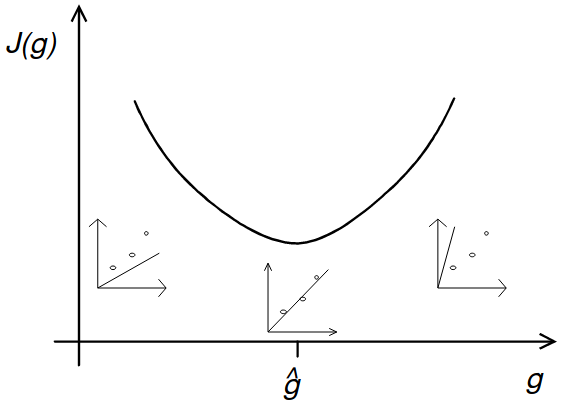
\includegraphics[width=0.5\textwidth]{img/least-aquare/Fcurve.png}
    \caption{Retas de ajuste mediante $\alpha$.}
    \label{fig:curvaF}
\end{wrapfigure}

$$
    J(\alpha) = \dfrac{1}{2}\sum_{i=1}^{n} (Y_i - \alpha X_i)^2
$$

\noindent O minimizante do funcional é obtido através da derivada em ordem ao parâmetro a estimar:
$$
    \dot{J}(\alpha) = \sum_{i=1}^{n} X_i(Y_i - \overline{\alpha} X_i) = 0
$$

\noindent A legitimidade do minimizante calculado é averiguada com recurso à segunda derivada\footnotemark[3]:
$$
    \ddot{J}(\alpha) > 0 
$$
\noindent\textbf{Nota 1}$\rightarrow$ A multiplicação de $J$ pelo escalar $1/2$ serve apenas para eliminar o termo 2 advindo da regra do expoente aquando a realização da derivada do funcional. Não influencia o cálculo do minimizante, já que estamos a igualar a derivada a 0.
\\\\
\noindent\textbf{Nota 2}$\rightarrow$ Para relações teórica que envolvam a estimação de mais do que um parâmetro, a segunda derivada deixa de ser um escalar, a legitimidade é assegurada mediante a matriz, que deve ser \underline{definida positiva}.

\footnotetext[3]{Assegura que a concavidade da curva do funcional está virada para cima, garantindo que $J(\alpha)$ seja um mínimo.}

\begin{theo}[\underline{Def.:} Matriz Definida Positiva]{}
   Se $\pmb{A}\, [n\times n]$ é uma matriz definida positiva, então os elementos da diagonal de $\pmb{A}$ são estritamente positivos, ou seja, $a_{ii} > 0, i = 1, \dots, n$. 
   
   \noindent \textbf{Nota:} Todos os valores próprios de $\pmb{A}$ são positivos ($\lambda_i > 0,\; \forall i \in \mathbb{N}$).
\end{theo}
%//==============================--@--==============================//%
\clearpage
\subsection[5.2 Notação Matricial]{$\rightarrow$ Notação Matricial}
Supondo uma equação às diferenças do género:
$$
    y(t) = a_1 y(t-1) + \dots + a_n y(t-n) = b_0 u(t-1) + \dots + b_m u(t - 1 - m)
$$
\noindent Define-se o vetor de parâmetros a estimar como:
$$
    \theta = \begin{bmatrix} a_1 & \dots & a_n & b_1 & \dots & b_n  \end{bmatrix}^\text{T}
$$
\noindent E o regressor como:
$$
    \varphi(t - 1) = \begin{bmatrix} -y(t-1) & \dots & -y(t-n) & u(t-1) & \dots & u(t-1-m)  \end{bmatrix}^\text{T}
$$
\noindent O modelo deduzido pode ser escrito como:

$$
    y(t) = \varphi(t - 1)\theta + \varepsilon(t) \rightarrow \text{Para n observações}
$$

$$
    \underbrace{\begin{bmatrix} y(1) \\ y(2) \\ \vdots \\ y(n) \end{bmatrix}}_{Y_e}= 
    \underbrace{\begin{bmatrix}  \varphi(0) \\ \varphi(1) \\ \vdots \\ \varphi(n - 1)\end{bmatrix}}_{\Phi}
    \begin{bmatrix} a_1 \\ a_2 \\ \vdots \\ a_n\end{bmatrix} + 
    \begin{bmatrix} \varepsilon(1) \\ \varepsilon(2) \\ \vdots \\ \varepsilon(n)\end{bmatrix}
$$

\noindent Onde $\varepsilon(t)$ é um resíduo que traduz a existência de erros experimentais, que se assumem (tipicamente) pequenos, deprezáveis. 
%//==============================--@--==============================//%
\subsection[5.3 Equação Normal]{$\rightarrow$ Equação Normal}
Consequentemente, a estimativa dos mínimos quadrados do vetor parâmetros $\theta$ do modelo acima descrito é por:
$$
    \Phi^{T}\Phi\bar{\theta} =  \Phi^{T}Y_e
$$

\noindent Denominada equação normal. Se $\Phi^{T}\Phi$ existir e for invertível então a estimativa dos mínimos quadrados existe e é única.
%//==============================--@--==============================//%

        \clearpage
    \section{6. Sistemas Distribuídos}
    %//==============================--@--==============================//%
\label{sec:SistemasDis}
\subsection[6.1 Problemas Representativos de PDE's]{$\rightarrow$ Problemas Representativos de PDE's}
Considere um troço de autoestrada em que se assumem verdadeiras as seguintes hipóteses:

\begin{itemize}
    \item[\ding{43}] Os veículos só podem entrar no início do troço e sair no final do troço.
    \item[\ding{43}] Os veículos não podem sair nem entrar ao longo do troço.
    \item[\ding{43}] Supõe-se que os veículos são suficientemente numerosos para que a densidade de tráfego (número de veículos por unidade de comprimento) seja uma variável contínua.
    \item[\ding{43}] No troço, todos os veículos deslocam-se sempre com uma velocidade constante
\end{itemize}

\noindent Seja $x$ a posição medida em Km a partir do início do troço e $\rho (x,t)$ a densidade de
tráfego (\textit{vehicle density}) no ponto de abcissa $x$, no instante $t$. Na prática, o que se mede é o fluxo de
tráfego $q(x,t)$ , dado pelo número de veículos por unidade de tempo que passam no
ponto de abcissa $x$ no instante $t$.

%//==============================--@--==============================//%

\subsubsection*{$\blacktriangle$ Sejam dois pontos de abcissas $\mathbf{x_2 > x_1}$ . Mostre que a densidade e o fluxo de
tráfego estão relacionados por:}

$$
\frac{\mathrm{d}}{\mathrm{d}t}\int_{x_1}^{x_2}\rho (x,t)dx = q(x_1,t) - q(x_2,t)
$$

\mdfsetup{linewidth=2pt}
\begin{mdframed}
    \noindent $\pmb{\rightarrow}$ \textbf{\textit{Densidade de tráfego (Vehicle density)}:}
     \textit{``The number of vehicles in a unit length of the road at time $t$ and position x. \textbf{A quantity that is easily recorded by observation of traffic flow along a road} is the flux of vehicles $q(x_i,t)$, defined as the number of vehicles that at time $t$ pass a given point with coordinate $x$ in a unit of time.''}
\end{mdframed}

\noindent O número de veículos num dado troço de autoestrada, caracterizado por dois pontos fixos $x_1$ e $x_2$ (onde $x_2$ > $x_1$), pode ser revisto como a diferença entre o fluxo de tráfego de entrada ($x_1$) e de saída ($x_2$) ( já que \textit{``Os veículos só podem entrar no início do troço e sair no final do troço.'')}:

$$
    \textbf{nº de veículos} = q(x_1,t) - q(x_2,t)
$$

\noindent A densidade de veículos no troço é a diferença de densidades entre o seu ponto inicial e final:

$$
    \rho(\Delta x, t) = \rho(x_2, t) - \rho(x_1, t) = \int_{x_1}^{x_2}\rho (x,t)dx
$$

\noindent Subsequentemente, trivialmente se reconhece que densidade de tráfego está subjugada à variação do número de veículos dentro do troço. A \textit{rate of change} da densidade tráfego entre os dois pontos (caracterizada pela derivada em ordem ao tempo do integral supramencionado) pode então ser relacionada com a diferença de fluxos de entrada e saída, tal como explicitado no enunciado.

%//==============================--@--==============================//%
\clearpage
\subsubsection*{$\blacktriangle$ Deduza uma equação às derivadas parciais para $\rho(x,t)$}

É possível obter um modelo simplificado do sistema fazendo um balanço de densidade da tráfego num troço da autoestrada de comprimento $\Delta x$ durante um intervalo $\Delta t$.

\vspace{-0.75em}
\begin{figure}[H]
    \centering
    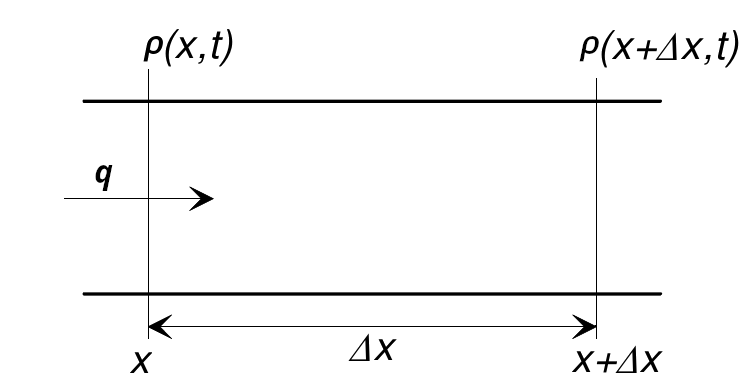
\includegraphics[width = 0.5\linewidth]{img/applied-dif-equ/fluxo-veiculo.png}
    \caption{Vizualização do balanço de densidade para um dado troço de autoestrada}
    \label{fig:fluxoV}
\end{figure}
\vspace{-1.5em}
$$
    \Delta x (\rho(x, t + \Delta t) - \rho(x, t)) = \Delta t (q(x,t) - q(x + \Delta x,t))
$$

\noindent Como $q = \text{v}\rho$ onde v é uma velocidade constante, é possível admitir que:
$$
    \Delta x (\rho(x, t + \Delta t) - \rho(x, t)) = \Delta t \cdot \text{v}(\rho(x,t) - \rho(x + \Delta x,t))
$$

\noindent Dividindo cada parcela da expressão por $\Delta x\Delta t$ e supondo que $\Delta x \to 0$ e $\Delta t \to 0$ obtém-se o modelo na forma de uma equação às derivadas parciais:% amo-te muito :3

$$
    \frac{\partial}{\partial t}\rho(x,t) = -\text{v}\frac{\partial}{\partial x}\rho(x,t)
$$

%//==============================--@--==============================//%
\subsubsection*{$\blacktriangle$ Por substituição na equação e verificação das condições iniciais, mostre que a
solução da equação deduzida é:}
$$
    \rho(x,t) = F(x - \text{v}t)
$$
\textbf{Em que $F(x) = \rho(x,0)$ é a densidade inicial de tráfego.}

\mdfsetup{linewidth=2pt}
\begin{mdframed}
    \noindent $\pmb{\rightarrow}$ Seguindo o método das características para PDE's quasilineares, a solução da equação pode ser vista como o deslocamento de veículos ao longo de um troço de autoestrada:

    $$
       \rho(x,t) = F\left(x - \int_{t_0}^{t}\text{v}\, dt, t_0\right) = 0
    $$
\end{mdframed}

\noindent Consequentemente, podemos provar a veracidade da solução através do uso da condição inicial:

$$
    \rho(x,0) = F\left(x - \int_{0}^{0}\text{v}\, dt, 0\right) = F(x)
$$

%//==============================--@--==============================//%
\clearpage
\subsubsection*{$\blacktriangle$ Mostre que ao longo das retas definidas no plano $[x,t]$ por $\frac{dx}{dt} = \text{v}$ a densidade
de tráfego é constante. Escreva a solução que dá $x$ como função de $t$
para estas rectas (denominadas rectas características. A partir daqui demonstre
a solução da equação às derivadas parciais dada na alínea anterior.}

Avaliando a \textit{rate of change} da densidade de tráfego ao longo do troço:
$$
    \frac{d}{d t}\rho(x,t) = \frac{\partial}{\partial t}\rho(x,t) + \frac{\partial}{\partial x}\rho(x,t)\cdot \frac{dx}{dt}
$$
Facilmente se depreende que os dois termos da parcela direita da equação se anulam:
$$
    \frac{d}{d t}\rho(x,t) = -\text{v}\frac{\partial}{\partial x}\rho(x,t) + \text{v}\frac{\partial}{\partial x}\rho(x,t) = 0
$$
\noindent Se a derivada total em ordem ao tempo (\textit{rate of change}) é nula, então não ocorrem variações ao longo do tempo e a densidade de tráfego é constante. Recorrendo agora à solução obtida na alínea anterior, o mesmo resultado é evidente:
$$
    \frac{d}{d t}\rho(x,t) = \frac{d}{d t}F(x - t) = F(x - \text{v}t)\frac{d}{d t} (x - \text{v}t) = F(x - \text{v}t)(\text{v} - \text{v}) = 0
$$
\noindent\textbf{A densidade de tráfego é constante} $\pmb{\rightarrow}$ A densidade de veículos no troço de autoestrada ao longo do tempo, para cada ponto de deslocamento é sempre a mesma.

%//==============================--@--==============================//%
\subsubsection*{$\blacktriangle$ Considere um troço de autoestrada com 20km e que a velocidade de
circulação é de 120km. Suponha que a densidade inicial de tráfego é definida por:}
\vspace{-1em}
$$
    \rho(x,0) = \begin{cases}
                    25 & 0 \le x \le 2\\
                    0  & x\notin [0,2]\\
                \end{cases}
$$
\noindent\textbf{Represente graficamente a densidade de tráfego em função do tempo no final
do troço. Suporte o seu resultado num desenho tridimensional no espaço}
\begin{itemize}
    \item[$\rightarrow$] A velocidade de circulação é constante, logo, a densidade de tráfego sofre um deslocamento linear para a direita ao longo do tempo.
    \item[$\rightarrow$] A densidade de tráfego não sofre alterações ao longo do troço de autoestrada, logo, a densidade de tráfego é idêntica à inicial para todos os pontos do troço.
\end{itemize}

\noindent O desenho tridimensional terá a seguinte forma:

\begin{figure}[H]
    \centering
    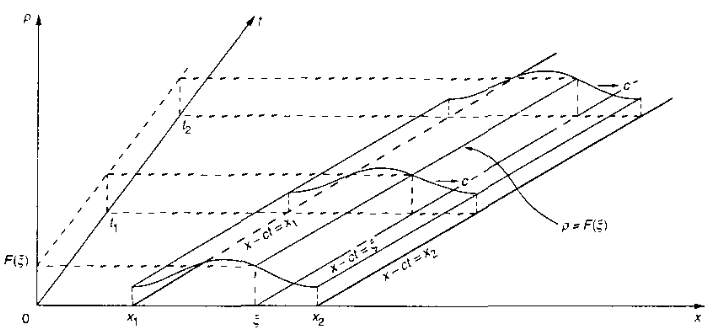
\includegraphics[width = 0.8\linewidth]{img/applied-dif-equ/plot3d.png}
    \caption{Solução geral do problema: $x_1 = 0$ e $p(x,0)$ igual à do enunciado.}
    \label{fig:3dplot}
\end{figure}

%//==============================--@--==============================//%

    
    %% refs
    \clearpage
    \bibliographystyle{unsrtnat}
    \nocite{*}
    {\footnotesize%
    \bibliography{refs}}
    %% attachments
    %\newpage
    %\input{appendix.tex}

\end{document}